\chapter{Results}

\section{Isothermal Jet}
Our first case involves the isothermal jet where both jet and ambient fluid are at $330 K$. Quantities of interest for this case are compared against incompressible round jet statistics as outlined in Pope \cite{Pope} and isothermal compressible jet turbulence features \cite{}. This case serves as a baseline for comparison with the other two cases involving non-isothermal jets. 
\subsection{Flow Field Features}
All images herein depict a slice of the 3D flow field at $z=0$. Each figure contains an instantaneous snapshot and a time-averaged snapshot of the entire slice domain, plus an additional zoomed-in image of the time-averaged quantity of interest near the inlet. All instantaneous images are taken from the final data point of the simulation.

Figure \ref{330_v_features} shows the axial velocity component of the flow field. The general spreading rate and decay of the velocity field can be seen from the instantaneous snapshot in \ref{330_v_1}. The flow is mostly steady up until $\nicefrac{y}{d}=2$ before perturbations begin. The stream mostly stays together through these initial perturbations up until $\nicefrac{y}{d}=5$ where spreading then begins. The averaged axial velocity fields in \ref{330_v_3} and \ref{330_v_4} shed more light on the approximate development regions of the jet. The potential core extends up to $\nicefrac{y}{d}=5$, followed by the transition region where $5 \leq \nicefrac{y}{d} \leq 15$, thereafter the jet appears fully developed. Centerline analysis of the turbulent kinetic energy later on will provide more information for these boundaries.  

\begin{figure}[htbp!]
\begin{subfigure}{0.25\textwidth}
	\centering
	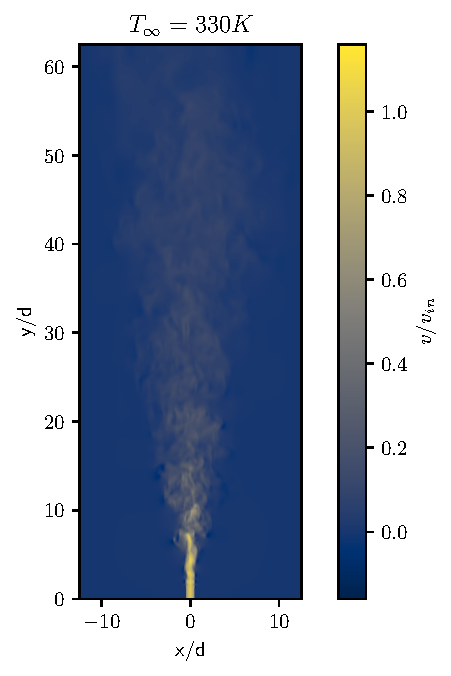
\includegraphics[scale=.65]{figures/Plots/vertical/330/v_scaled_vert_330.pdf}
	\caption{Scaled instantaneous axial velocity} \label{330_v_1}
\end{subfigure}
\hfill
% \begin{subfigure}{0.3\textwidth}
% 	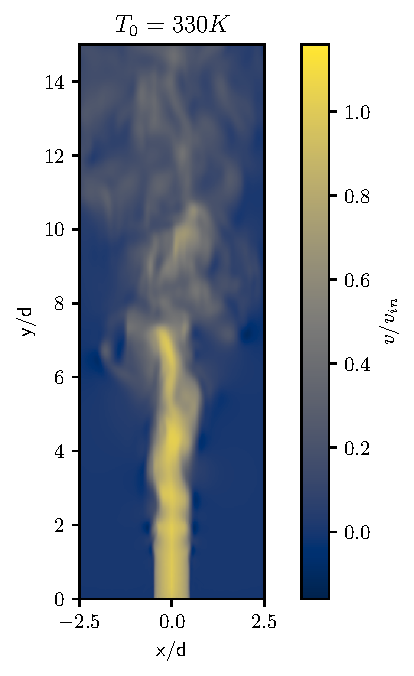
\includegraphics[scale=.75]{figures/Plots/vertical/330/v_scaled_vert_330_zoom.pdf}
% 	\caption{Close up of scaled instantaneous axial velocity near inlet} \label{330_v_2}
% \end{subfigure}
\begin{subfigure}{0.25\textwidth}
	\centering
	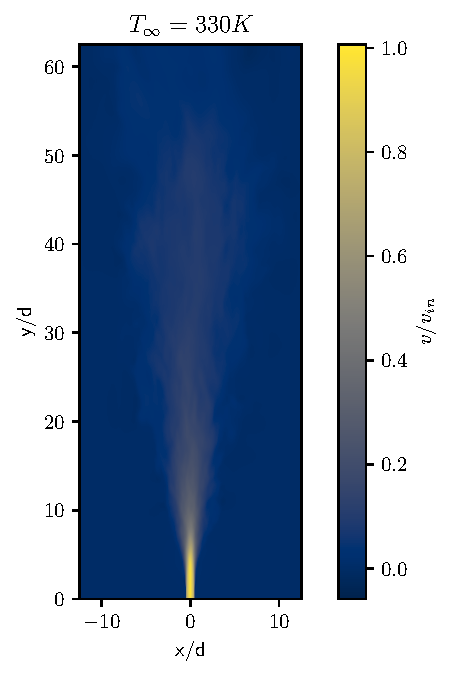
\includegraphics[scale=.65]{figures/Plots/vertical/330/v_scaled_vert_avg_330.pdf}
	\caption{Scaled average axial velocity} \label{330_v_3}
\end{subfigure}
\hfill
\begin{subfigure}{0.25\textwidth}
	\centering
	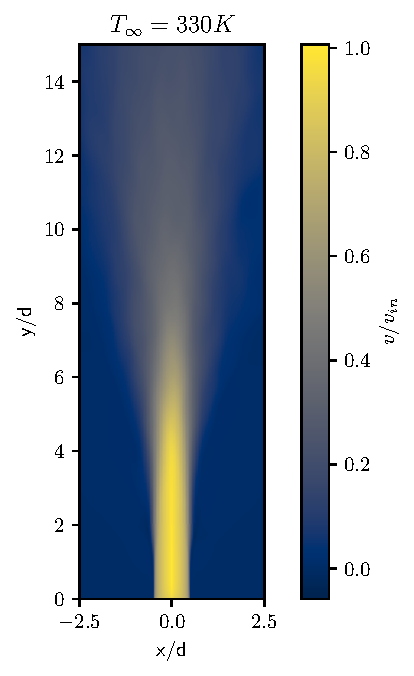
\includegraphics[scale=.65]{figures/Plots/vertical/330/v_scaled_vert_avg_330_zoom.pdf}
	\caption{Close up of scaled average axial velocity near inlet} \label{330_v_4}
\end{subfigure}
\caption{Axial velocity features of the isothermal jet}
\label{330_v_features}
\end{figure}

Figure \ref{330_pressure_features} shows minor pressure fluctuations in the flow, scaled against the maximum pressure achieved above the ambient pressure. \ref{330_pressure_1} shows minor pressure oscillations mirrored on each side of the jet edge in the same zone as the initial velocity fluctuations see in \ref{330_v_1}. Thereafter, the oscillations become off-kilter, correlating to the beginning of the jet disintegration as seen in the velocity field. Pressure fluctuations are concentrated near the inlet and die down past the transition zone. This can be seen more clearly in \ref{330_pressure_3}. On average, pressure fluctuations yield a minor increase within the potential core and decrease on the jet perimeter, as can be seen in \ref{330_pressure_4}. Fluctuations also lead to a minor pressure drop on average in the transition region.  

\begin{figure}[htbp!]
\begin{subfigure}{0.25\textwidth}
	\centering
	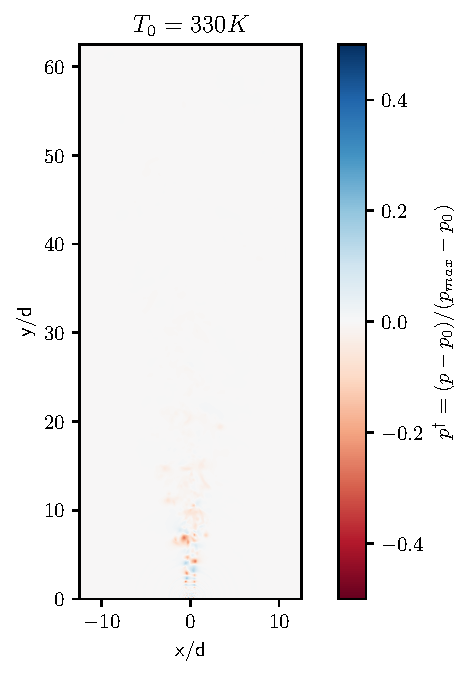
\includegraphics[scale=.65]{figures/Plots/vertical/330/pressure_scaled_vert_330.pdf}
	\caption{Scaled instantaneous pressure fluctuations} \label{330_pressure_1}
\end{subfigure}
\hfill
% \begin{subfigure}{0.25\textwidth}
% 	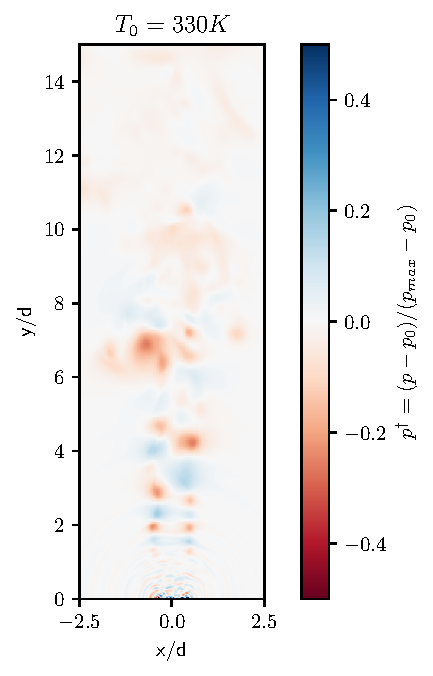
\includegraphics[scale=.65]{figures/Plots/vertical/330/pressure_scaled_vert_330_zoom.pdf}
% 	\caption{Close up of scaled instantaneous pressure fluctuations near inlet} \label{330_pressure_2}
% \end{subfigure}
\begin{subfigure}{0.25\textwidth}
	\centering
	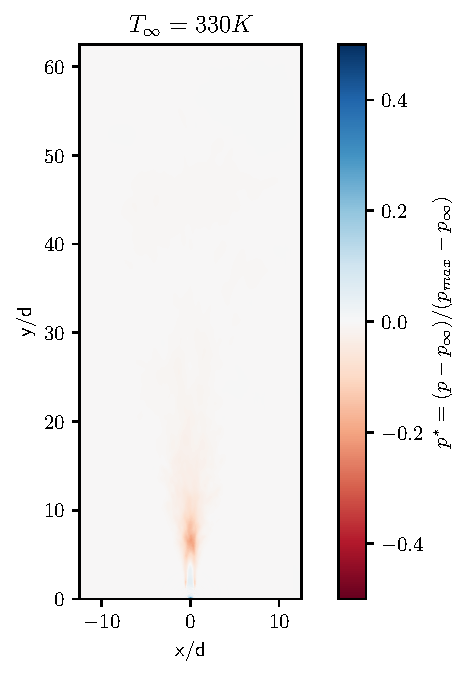
\includegraphics[scale=.65]{figures/Plots/vertical/330/pressure_scaled_vert_avg_330.pdf}
	\caption{Scaled average pressure fluctuations} \label{330_pressure_3}
\end{subfigure}
\hfill
\begin{subfigure}{0.25\textwidth}
	\centering
	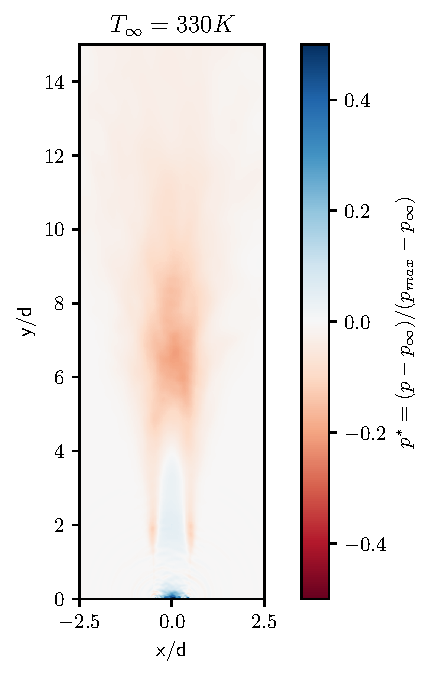
\includegraphics[scale=.65]{figures/Plots/vertical/330/pressure_scaled_vert_avg_330_zoom.pdf}
	\caption{Close up of scaled average pressure fluctuations near inlet} \label{330_pressure_4}
\end{subfigure}
\caption{Pressure features of the isothermal jet}
\label{330_pressure_features}
\end{figure}

Figure \ref{330_magvort_features} shows magnitude of the vorticity scaled between the maximal and minimal values. \ref{330_magvort_1} shows the strongest vorticity occurring at the jet interface with the ambient fluid near the inlet. Past this initial stage, vortex shedding occurs and vorticity dissipates as the jet spreads. The averages in \ref{330_magvort_3} and \ref{330_magvort_4} both show again that the most intense vorticity occurs at the inlet along the outer edge of the jet. This high intensity remains constant until about $\nicefrac{y}{d}=1$ before more mixing with the ambient fluid occurs as the jet spreads and the vorticity lessens in intensity. Vortices are still restricted to the jet edge until around $\nicefrac{y}{d} = 5$ where the transition to fully developed turbulence enables vortical motions to extend across the fully spread of the jet. 

\begin{figure}[htbp!]
\begin{subfigure}{0.25\textwidth}
	\centering
	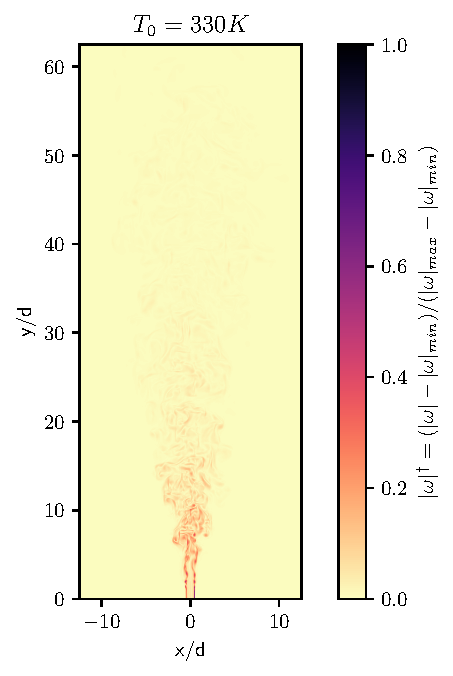
\includegraphics[scale=.65]{figures/Plots/vertical/330/magvort_scaled_vert_330.pdf}
	\caption{Scaled instantaneous vorticity magnitude} \label{330_magvort_1}
\end{subfigure}
\hfill
% \begin{subfigure}{0.25\textwidth}
%	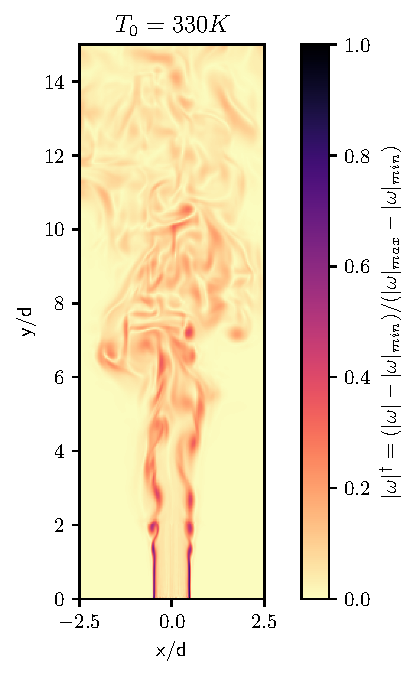
\includegraphics[scale=.65]{figures/Plots/vertical/330/magvort_scaled_vert_330_zoom.pdf}
%	\caption{Close up of scaled instantaneous vorticity magnitude near inlet} \label{330_magvort_2}
%\end{subfigure}
\begin{subfigure}{0.25\textwidth}
	\centering
	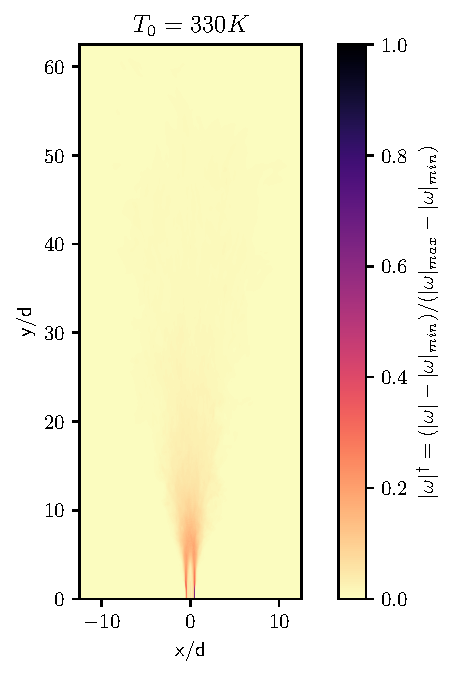
\includegraphics[scale=.65]{figures/Plots/vertical/330/magvort_scaled_vert_avg_330.pdf}
	\caption{Scaled average vorticity magnitude} \label{330_magvort_3}
\end{subfigure}
\hfill
\begin{subfigure}{0.25\textwidth}
	\centering
	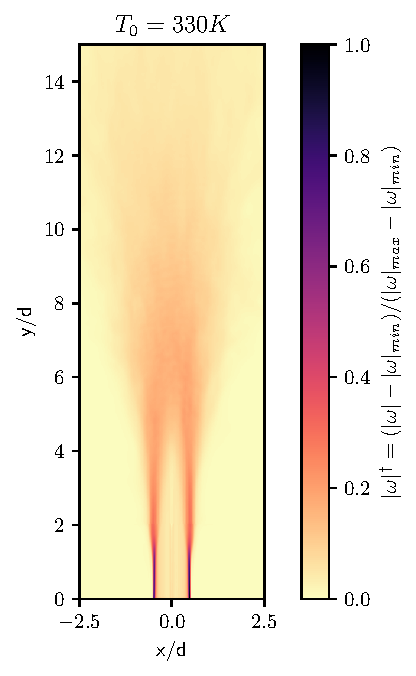
\includegraphics[scale=.65]{figures/Plots/vertical/330/magvort_scaled_vert_avg_330_zoom.pdf}
	\caption{Close up of scaled average vorticity magnitude near inlet} \label{330_magvort_4}
\end{subfigure}
\caption{Vorticity magnitude features of the isothermal jet}
\label{330_magvort_features}
\end{figure}

\subsection{Mean Flow Properties}
Figure \ref{330_centerline_decay} depicts the time and radially averaged scaled axial velocity component plotted against radial distance from the centerline at multiple normal slices downstream from the inlet. The velocity is scaled by the average axially velocity value at the inflow while the radial direction is scaled by the jet diameter. These plots demonstrate the axially velocity decay as the flow progresses further downstream. As velocity value along the centerline decreases, the overall velocity profile also widens and flattens out. Typically, for the round turbulent jet, this expansion would occur in such a way that upon specially selected scaling, these profiles would collapse into one profile after a certain point. This potential is explored further in the next figure. Here though this decay is a common feature of how the axial velocity of the jet develops as it leaves the inlet. 

\begin{figure}[htbp!]
\begin{center}
	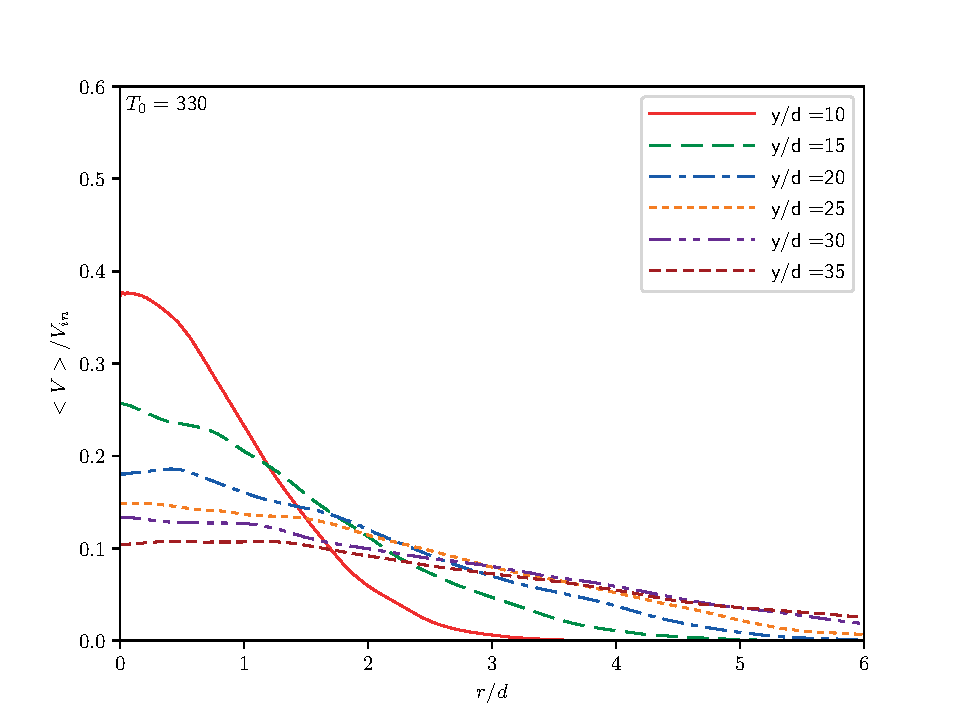
\includegraphics[scale=.7]{figures/Plots/radial/slices_5/same_ambient/ur_u_in_vs_r_d.pdf}
	\caption{Average (both in time and radially) axial velocity scaled by inlet value plotted along radial distance from centerline. Profile decay follows similar trajectory to what is expected in incompressible round jet theory \cite{Pope}.} \label{330_centerline_decay}
\end{center}
\end{figure}

Figure \ref{330_r_v_features} depicts time and radially averaged scaled axial velocity components plotted against the radial distance from the centerline. Each curve is made at a slice normal to the axial flow direction at different points downstream. Figure \ref{330_r_vs_v_1} depicts velocity curves every $3d$ downstream from the inlet near where the transition region begins while Figure \ref{330_r_vs_v_2} contains plots taken every $5d$. The axial velocity is scaled by the centerline value $v_c$ while the radial distance is scaled by the half width half mean (HWHM), where the velocity component is equal to half the value on the centerline $v(r_{1/2}) = \nicefrac{v_c}{2}$.

Figure \ref{330_r_vs_v_1} shows the near-field axial velocity profiles. They already exhibit self-similarity collapse into one profile which is most likely the result of the inflow condition \cite{}. In the far-field slices of \ref{330_r_vs_v_2}, self-similarity is fairly well maintained with minor fluctuations in the center and edge of the jet. These fluctuations are most likely the result of low resolution in the time averaging of available data. 

\begin{figure}[htbp!]
\begin{center}
\begin{subfigure}{0.45\textwidth}
	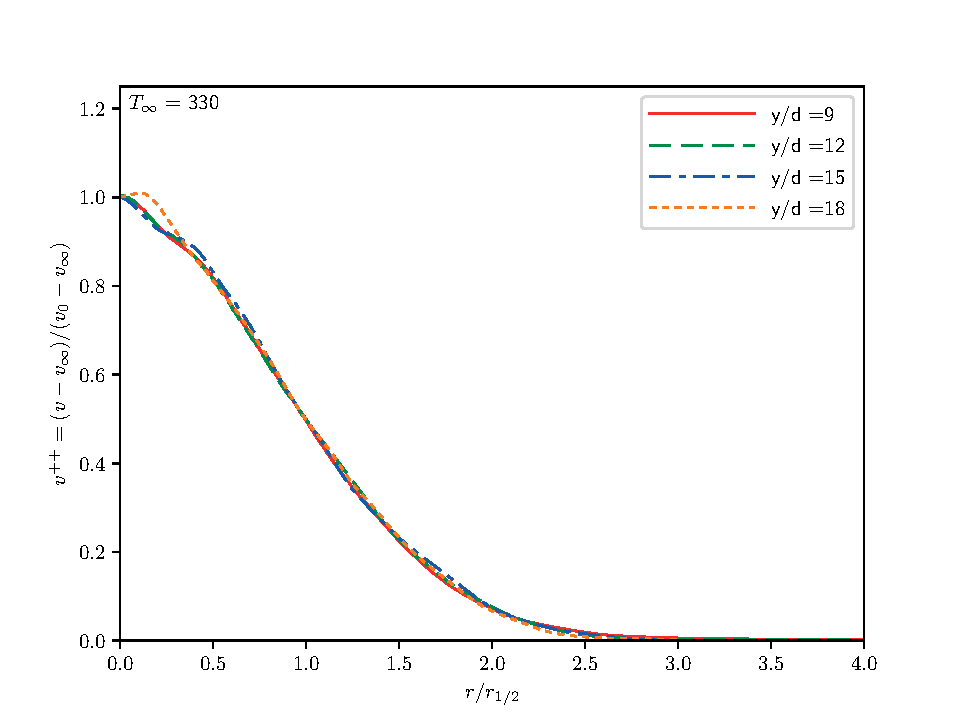
\includegraphics[scale=.45]{figures/Plots/radial/slices_3/same_ambient/r_vs_v.pdf}
	\caption{Near-Field} \label{330_r_vs_v_1}
\end{subfigure}
\begin{subfigure}{0.45\textwidth}
	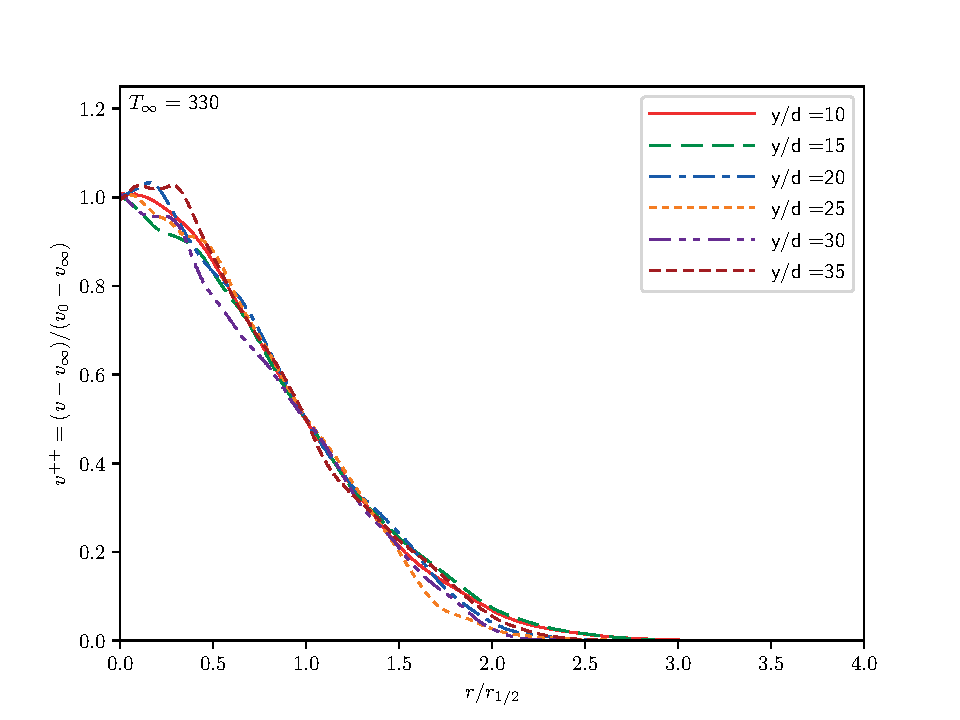
\includegraphics[scale=.45]{figures/Plots/radial/slices_5/same_ambient/r_vs_v.pdf}
	\caption{Far-Field} \label{330_r_vs_v_2}
\end{subfigure}
\caption{Normal slices of scaled axial velocity, averaged in both time and the radial direction. Plotted against radial direction scaled by $r_{1/2}$. Both near- and far-field regions demonstrate the self-similarity within the round turbulent jet.}
\label{330_r_v_features}
\end{center}
\end{figure}

Another common feature of round turbulent jets is the development of a linear relationship between the jet centerline value and the distance downstream. This comparison is depicted in Figure \ref{330_centerline_scaling}. Here, the centerline value of the axial velocity $v_0$ is inversely linearly proportional to the distance downstream. The dip at $\nicefrac{y}{d}=30$ may be attributed to again lack of convergence due to low sample size in time averaging. 

\begin{figure}[H]
\begin{center}
	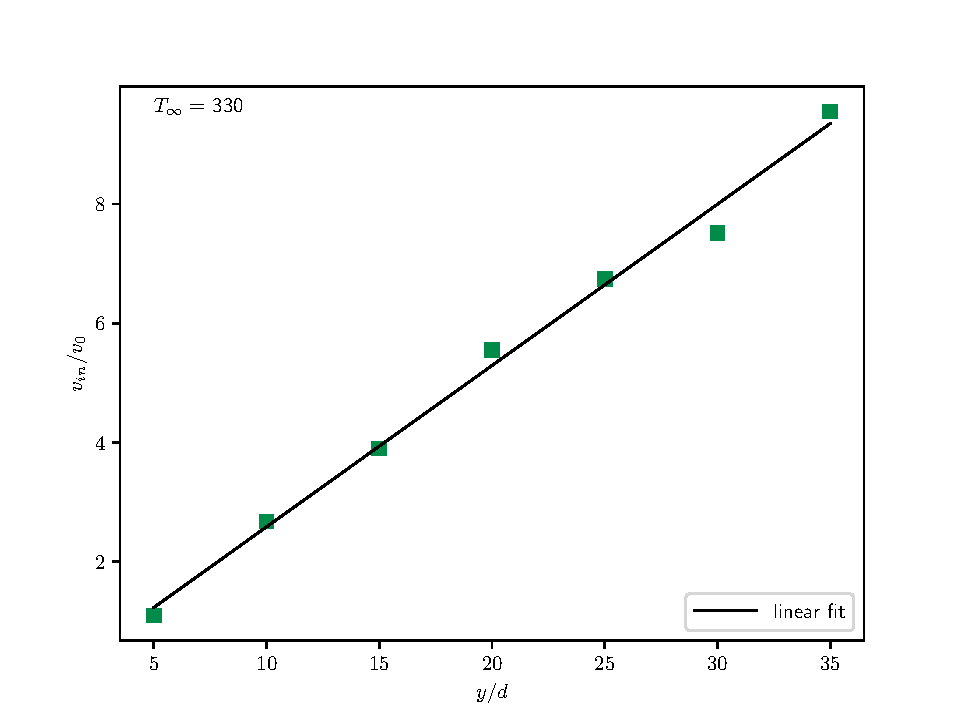
\includegraphics[scale=.7]{figures/Plots/radial/slices_5/same_ambient/uin_u0_vs_x_d.pdf}
	\caption{Axial inlet velocity scaled by centerline values along the axial direction. When distance downstream is scaled by jet diameter, linear decay of the centerline axial velocity is observed.} \label{330_centerline_scaling}
\end{center}
\end{figure}

\subsection{Turbulence Dynamics}
Figure \ref{330_reynolds_features} shows the time and radially averaged Reynolds stresses at two points downstream from the inlet. Here, velocity components $(u,v,w)$ correspond to the $(r,y,\theta)$ directions, respectively. Each Reynolds stress component follows general trends associated with round turbulent jets \cite{Pope}, with the axial component providing the leading contribution, followed by the other two directional components closely with these two being of roughly the same magnitude, and the cross-directional component contributing the least. The cross-directional component is non-zero at the jet center; this could be due to... Note also that self-similarity is not exhibited, as each component exhibits an increase in magnitude at the center of the jet as distance downstream is increased. 

\begin{figure}[hbtp!]
\begin{center}
\begin{subfigure}{0.45\textwidth}
	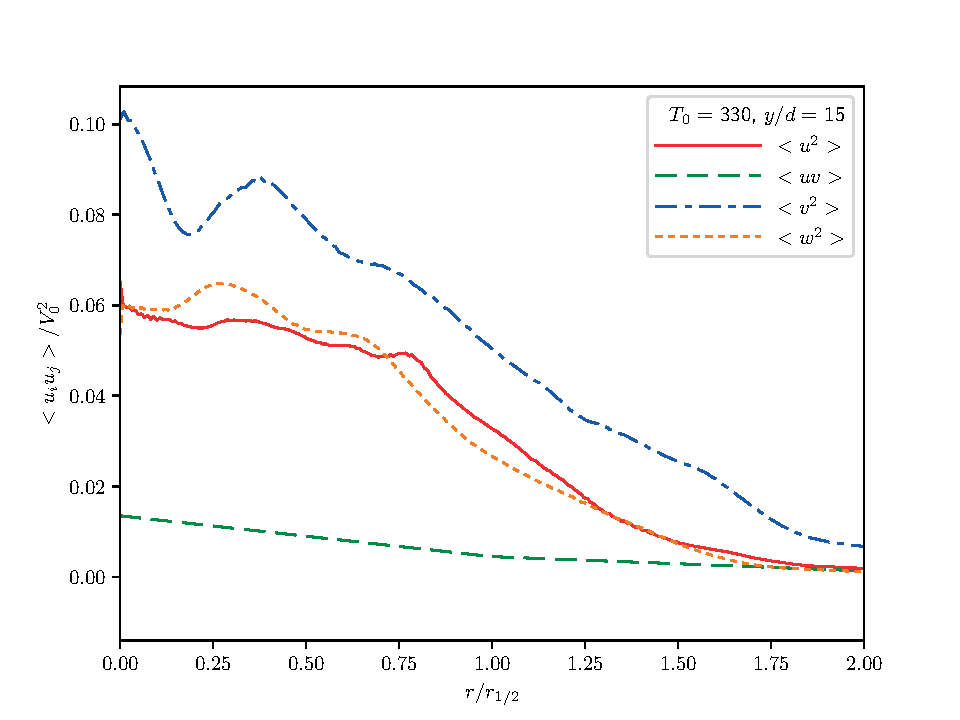
\includegraphics[scale=.45]{figures/Plots/radial/slices_5/same_ambient/Rey_Stress_0_15.pdf}
	\caption{Reynolds stresses at $y/d=15$} \label{330_rey_15}
\end{subfigure}
\begin{subfigure}{0.45\textwidth}
	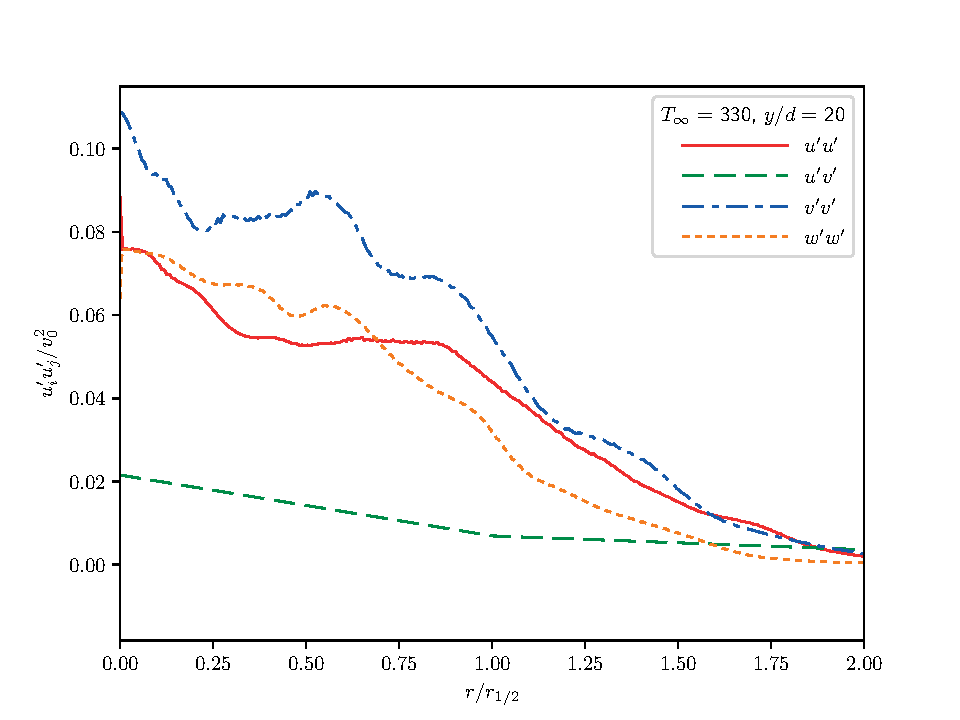
\includegraphics[scale=.45]{figures/Plots/radial/slices_5/same_ambient/Rey_Stress_0_2.pdf}
	\caption{Reynolds stresses at $y/d=20$} \label{330_rey_20}
\end{subfigure}
\caption{Time and radially averaged Reynolds stresses for the isothermal jet at two locations downstream. Both slices follow similar Reynolds stress relations as seen in incompressible round jet \cite{Pope}.}
\label{330_reynolds_features}
\end{center}
\end{figure}

Figure \ref{330_TKE_features} shows the time average turbulent kinetic energy components along the centerline of the jet. Each component grows through the potential core region of the jet up until all components reach a peak in energy around $\nicefrac{y}{d}=6$, with the axial component's peak coming slightly ahead of the other two directions. Rapid decay is then observed up until around $\nicefrac{y}{d} = 15$ before a slower decay sets in up until a leveling off is achieved around $\nicefrac{y}{d} = 30$. This rapid decay and then further progression correspond to the transition and fully developed jet regions, respectively.   

\begin{figure}[hbtp!]
\begin{center}
	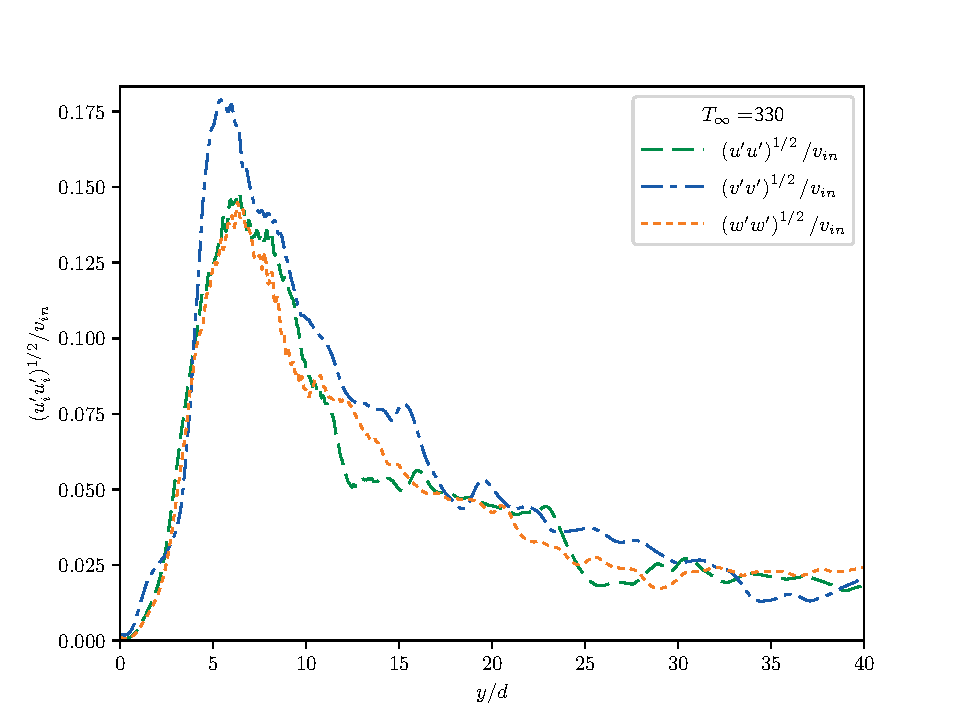
\includegraphics[scale=.7]{figures/Plots/centerline/330_TKEuvw_centerline.pdf}
	\caption{Average turbulent kinetic energy components along centerline.} \label{330_TKE_features}
\end{center}
\end{figure}

\section{Non-Isothermal Jets}
The two non-isothermal jet cases as described in Chapter 4 are presented here. Some features are compared to the isothermal jet case while others are used for direct comparison between the two non-isothermal cases. Again, the $350 K$ ambient case depicts a jet entering a warmer ambient fluid, moving further away from the supercritical point while the $314 K$ ambient case depicts a jet entering a cooler ambient fluid with a transition over the pseudo-boiling point. It is anticipated that the $314 K$ ambient case will then vary much more prominently from the other two cases across various quantities of interest examined. 
\subsection{Flow Field Features}
Figure \ref{all_v_features} shows various axial velocity field comparisons between both the isothermal and non-isothermal jets. The instantaneous axial velocity over the whole domain is depicted in \ref{all_v_1}. The $350 K$ ambient case has a laminar flow region of similar length to the $330 K $ ambient case, with the jet core staying in tact up until $\nicefrac{y}{d} = 2$ before fluctuations begin to take effect. The developing region after this within $5 \leq \nicefrac{y}{d} \leq 15$ appears to be slightly more volatile in the $350 K$ ambient case compared to the $330 K$ ambient case, with the region containing finer-scale fluctuations. The spreading rate of the $350 K$ ambient case is smaller than that of the base case while overall intensity levels seem to be comparable in the downstream direction. The $314 K$ ambient case has a much shorter laminar region compared to the base case, with fluctuations beginning to become apparent at $\nicefrac{y}{d} = 1$. Perturbations after that appear to be more symmetric in structure, with vorticies along the jet edge staying in tandem instead of the oscillatory shedding apparent in the other two cases. The $314 K$ ambient case also appears to have a spreading rate comparable to the $350 K$ ambient case, but with a faster decay in intensity in the downstream direction. \ref{all_v_2} helps further illuminate the difference in spread of the three jets. Here the $350 K$ ambient core intensity is more persistent downstream with a more distinct and thinner outer edge flow present than in the $330 K$ ambient case, while the $314 K$ case has a lower intensity central flow region but a comparably sized edge flow region compared to the $330 K$ ambient case. Finally, \ref{all_v_3} helps depict the potential core and transition regions of the three cases more clearly. Here, the similarity between the potential cores of the $330 K$ and $350 K$ ambient cases is clear while the $314 K$ ambient case has a much shorter core length. 

\begin{figure}[H]
\begin{subfigure}{0.5\textwidth}
	\centering
	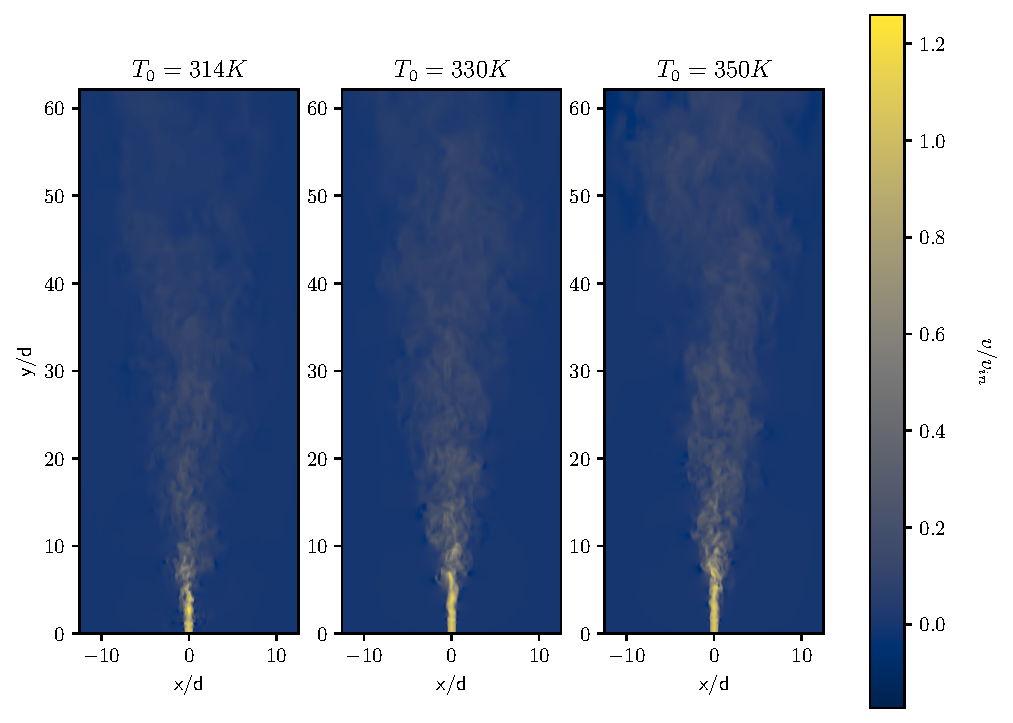
\includegraphics[scale=.45]{figures/Plots/vertical/v_scaled_vert_all.pdf}
	\caption{Instantaneous axial velocity field.} \label{all_v_1}
\end{subfigure}
\hfill
\begin{subfigure}{0.5\textwidth}
	\centering
	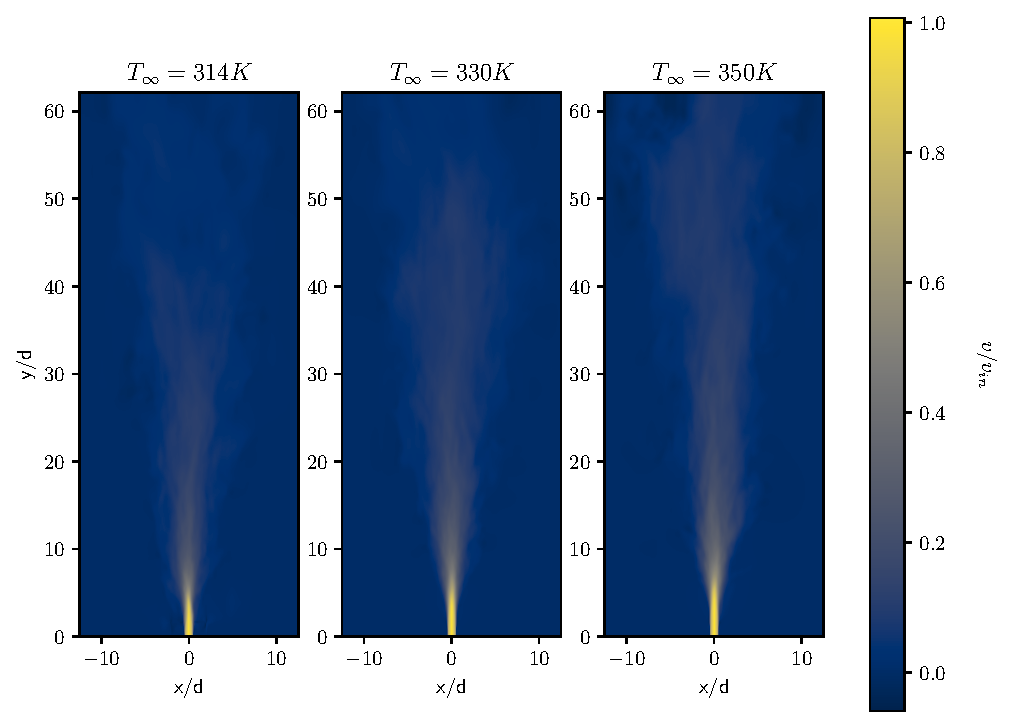
\includegraphics[scale=.45]{figures/Plots/vertical/v_scaled_vert_avg_all.pdf}
	\caption{Average axial velocity field.} \label{all_v_2}
\end{subfigure}
\vfill
\centering
\begin{subfigure}{0.5\textwidth}
	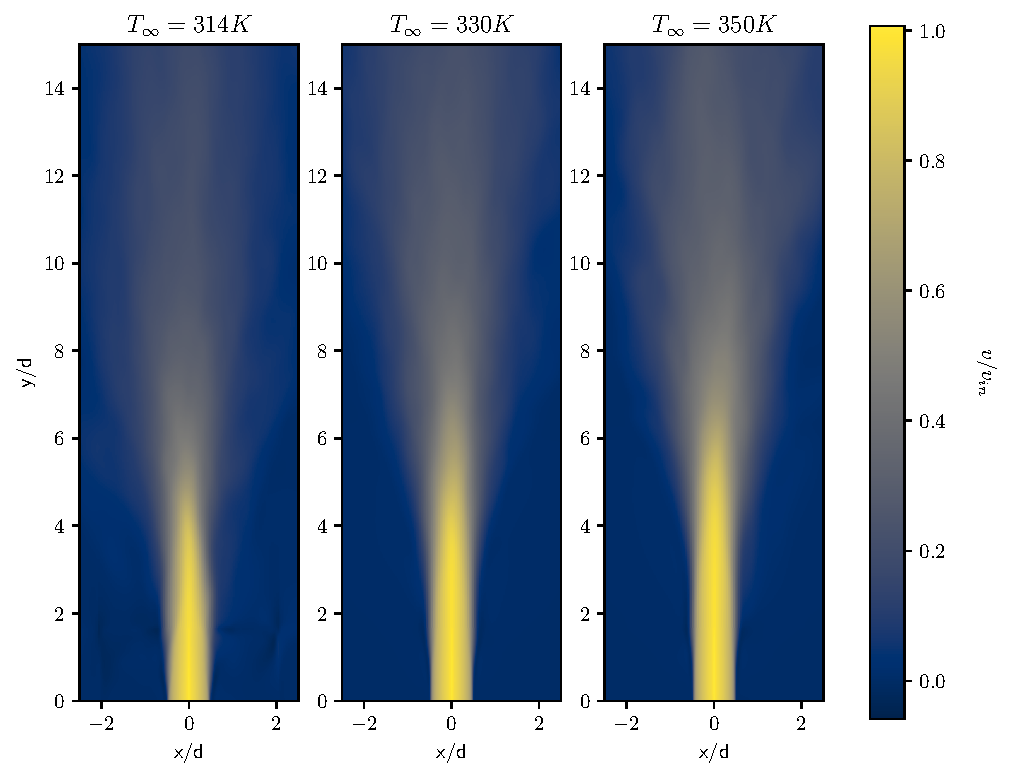
\includegraphics[scale=.45]{figures/Plots/vertical/v_scaled_vert_avg_all_zoom.pdf}
	\caption{Average axial velocity near inlet.} \label{all_v_3}
\end{subfigure}
\caption{Axial velocity field comparison between 314K ambient case (left), 330K ambient case (middle), and 350K ambient case (right).}
\label{all_v_features}
\end{figure}

Figure \ref{all_pressure_features} shows pressure fluctuations near the inlet for all three cases. \ref{all_pressure_1} contains an instantaneous snapshot of these fluctuations near the inlet. The $350 K$ ambient case is comparable to the $330 K$ ambient case, with similar large coherent structures forming in the pressure oscillations. However, the initial pressure waves emanating from the inlet are stronger in the $350 K$ ambient case, resulting in slightly more intense fluctuations downstream. Minor spurious perturbations are also seen downstream in the $350 K$ ambient case. The $314 K$ ambient case is qualitatively much different from the other two cases. Larger coherent structures are much less defined, with smaller fluctuations appearing much more prominent throughout. There is also a band of cells slightly before $\nicefrac{y}{d}=2$ where perturbations are more concentrated. This could be due to... some sort of gls{amr} issue? *(this is right around where the grid refinement drops from the imposed high-level refinement at the inlet)* Average pressure fluctuation can be seen in \ref{all_pressure_2}. All cases have a slight increase in pressure isolated within the potential core surrounded by and followed with a pressure drop. The difference between these low and high pressure pockets is most prominent in the $314 K$ ambient case, followed by the $330 K$ ambient case. Numerical artifacts are extremely prominent in the $314 K$ ambient case, most likely due to.... with some similar artifacts present in the $350 K$ ambient case as well.  

\begin{figure}[H]
\begin{subfigure}{0.5\textwidth}
	\centering
	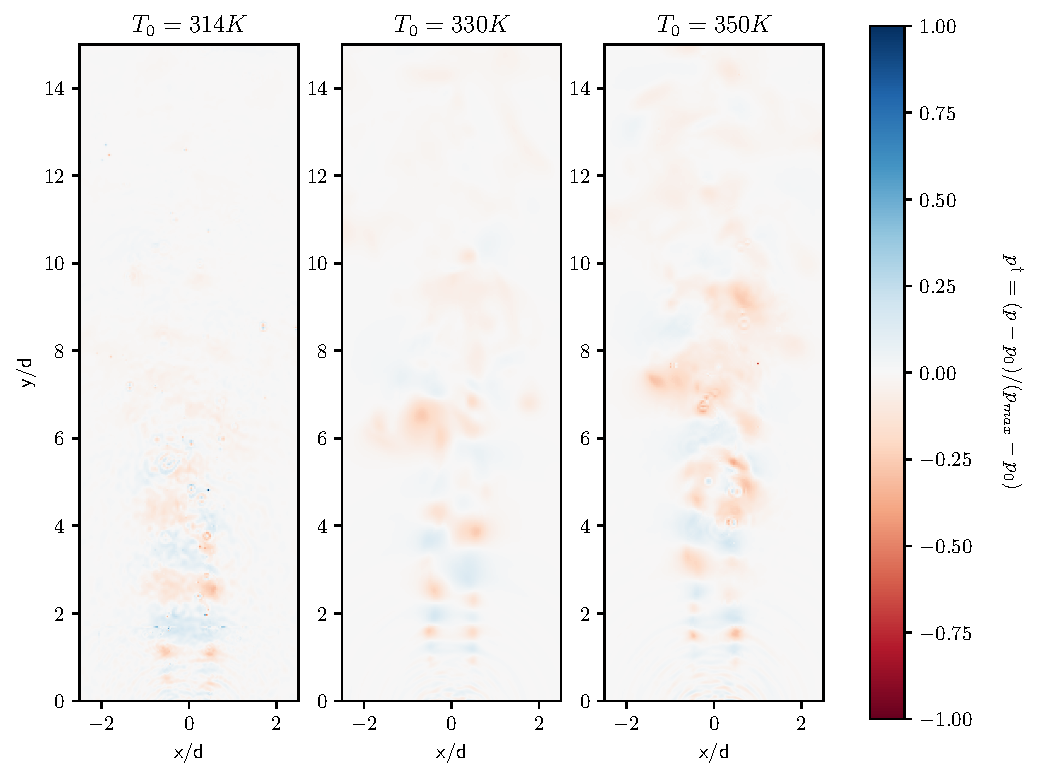
\includegraphics[scale=.45]{figures/Plots/vertical/pressure_scaled_vert_all_zoom.pdf}
	\caption{Instantaneous pressure fluctuations near inlet.} \label{all_pressure_1}
\end{subfigure}
\hfill
\begin{subfigure}{0.5\textwidth}
	\centering
	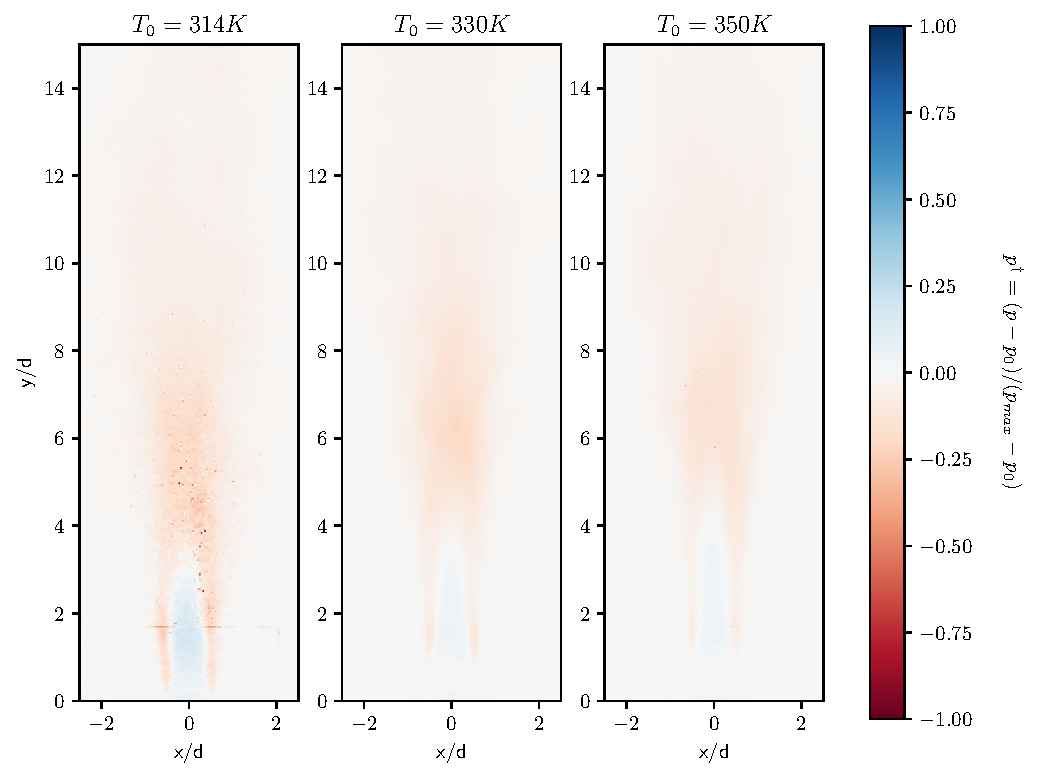
\includegraphics[scale=.45]{figures/Plots/vertical/pressure_scaled_vert_avg_all_zoom.pdf}
	\caption{Average pressure fluctuations near inlet.} \label{all_pressure_2}
\end{subfigure}
\caption{Pressure fluctuation field comparison between 314K ambient case (left), 330K ambient case (middle), and 350K ambient case (right).}
\label{all_pressure_features}
\end{figure}

Figure \ref{all_magvort_features} shows both instantaneous and time-averaged flow fields of the vorticity magnitude for the three cases. The vorticity magnitude features seen in \ref{all_magvort_1} follow similar trends as were established with the axial velocity discussion in Figure \ref{all_v_1}. In all three cases, the strongest vorticity occurs along the jet edge right at the inflow, leading to vortex formation and subsequent fluctuations. This steady inflow window before fluctuations lead to jet disintegration is comparable between the $330 K$ and $350 K$ ambient case. However, the $350 K$ maintains higher vorticity intensity downstream with pockets of stronger vorticity seen in the transition region of the jet compared to that of the $330 K$ ambient case. The $314 K$ ambient case has a shorter region of steady flow in and also features more prominently distinct vortex formation along the edge of the jet. These vortices roll along the edge in tandem before mixing to lead into the transition region around $\nicefrac{y}{d} = 3$. Similar to what was seen with the $314 K$ ambient pressure field, there are some vorticity artifacts present in the mesh at the edge of the initial high-refinement zone surrounding the jet inlet. Similar to the $350 K$ ambient case, the $314 K$ ambient case also maintains some pockets of high vorticity, but then does an overall decay downstream that is much more intense than the other two cases. The averaged vorticity magnitude fields in \ref{all_magvort_2} and \ref{all_magvort_3} help showcase the different jet regions and jet spreading. From \ref{all_magvort_2} one can see that the $350 K$ ambient case has more widespread vorticity in the transition region from around $5 \leq \nicefrac{y}{d} \leq 15$ and then maintains the intensity formed here for further along downstream compared to the $330 K$ ambient case. The $314 K$ ambient case has a much narrower vorticity range in the same region with intensity decaying much more rapidly downstream. Near the inlet, as depicted in \ref{all_magvort_3}, it's easier to see that the $314 K$ ambient case begins spreading much earlier than the other two cases and has much less uniform vorticity along the jet edges. These vorticity fluctuations before the mesh refinement change may contribute to the vorticity artifacts seen? This earlier breakup also impacts the way the high-vorticity outer edges of the jet merge around the low-vorticity center at the end of the potential core, where the merging of the two jet edges across the middle meet in an almost concave point as compared to the more convex central region seen in the other two cases. 

\begin{figure}[htbp!]
\begin{subfigure}{0.5\textwidth}
	\centering
	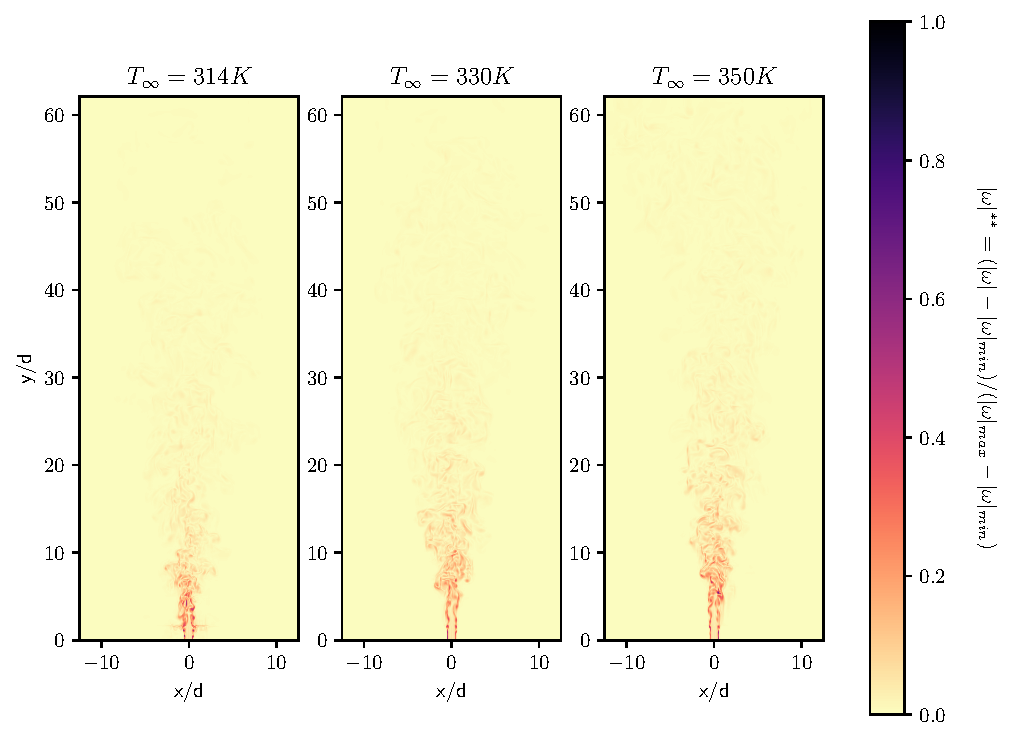
\includegraphics[scale=.45]{figures/Plots/vertical/magvort_scaled_vert_all.pdf}
	\caption{Instantaneous vorticity magnitude field.} \label{all_magvort_1}
\end{subfigure}
\hfill
\begin{subfigure}{0.5\textwidth}
	\centering
	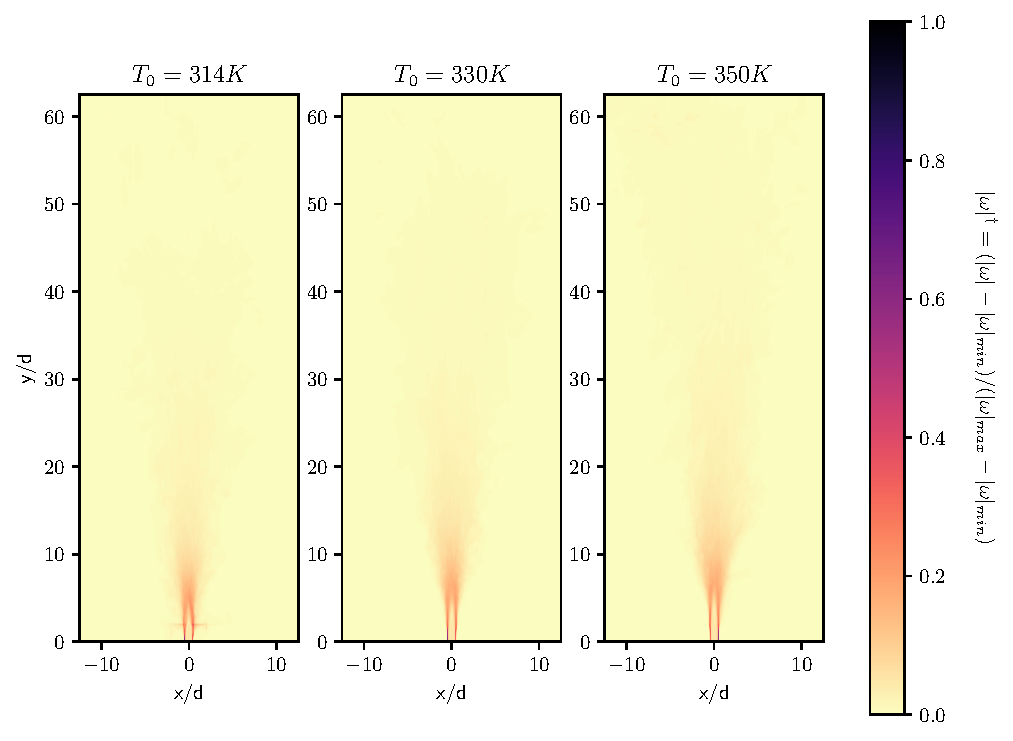
\includegraphics[scale=.45]{figures/Plots/vertical/magvort_scaled_vert_avg_all.pdf}
	\caption{Average vorticity magnitude field.} \label{all_magvort_2}
\end{subfigure}
\vfill
\centering
\begin{subfigure}{0.5\textwidth}
	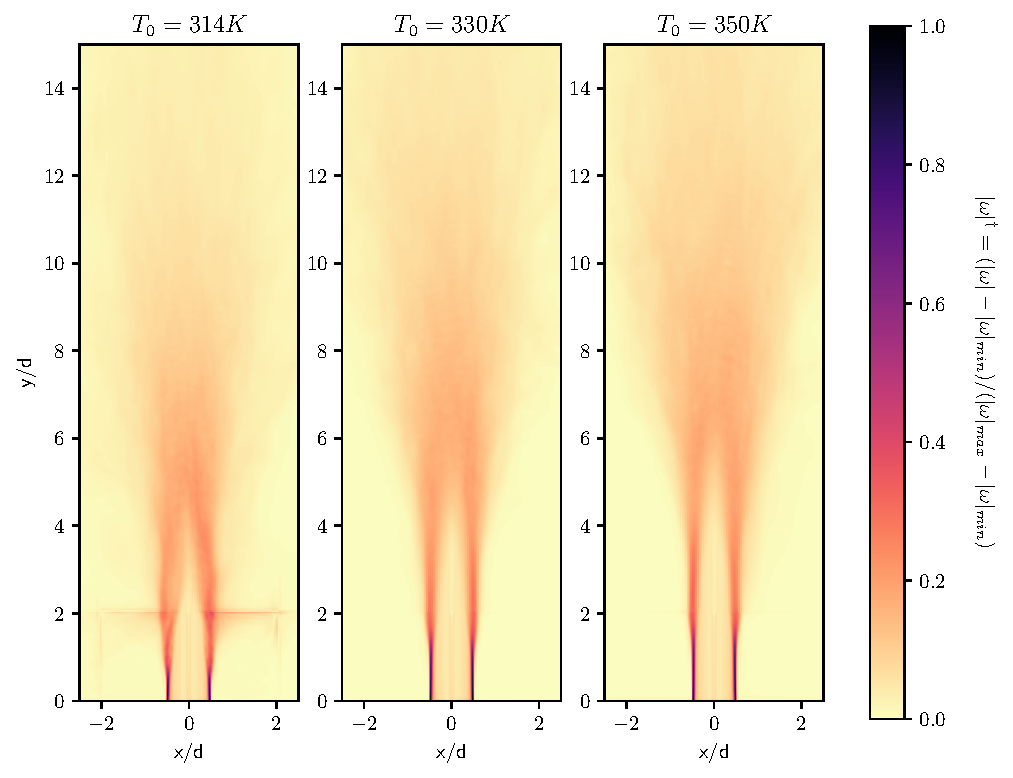
\includegraphics[scale=.45]{figures/Plots/vertical/magvort_scaled_vert_avg_all_zoom.pdf}
	\caption{Average vorticity magnitude near inlet.} \label{all_magvort_3}
\end{subfigure}
\caption{Vorticity magnitude field comparison between 314K ambient case (left), 330K ambient case (middle), and 350K ambient case (right).}
\label{all_magvort_features}
\end{figure}

The final figure in this section, Figure \ref{noniso_various_features}, contains direct comparisons between the two non-isothermal cases for various quantities of interest. Figure \ref{noniso_temp_1} shows temperature change between the jet and the ambient fluid. The jet more rapidly approaches the ambient fluid temperature in the $314 K$ ambient case as compared to the $350 K$ ambient case, where temperature variation from the inlet is much more gradual downstream. Figure \ref{noniso_cp_1} shows the constant-pressure specific heat variation between the two cases. The added peak in specific heat can be seen in the $314 K$ ambient case as the fluid transitions through the pseudo-boiling point. This peak occurs at the jet edge in the potential core and is additionally maintained after the transition region, showing a slower transition to the ambient specific heat as compared to the $350 K $ ambient case. \ref{noniso_rho_1} shows the density transition between the jet and the ambient fluid. Density change downstream in both cases occurs at similar rates, with both jets exhibiting a rapid shift during the transition region and then continuing with a much slower adjustment thereafter. The last group of images, \ref{noniso_Cs_1}, \ref{noniso_Hi_1}, and \ref{noniso_Z_1}, show the sound speed, enthalpy, and compressibility factor of the fluid, respectively. All three quantities exhibit similar trends, with the $350 K$ ambient case showing a more rapid transition to the ambient conditions as compared to the $314 K$ ambient case. These follow the same trend as seen in the temperature, but to varying degrees of intensity. For example, enthalpy appears to have an overall faster downstream decay for both cases as compared to the temperature decay, while sound speed and compressibility factor have comparable decay rates. 

\begin{figure}[H]
\begin{subfigure}{0.5\textwidth}
	\centering
	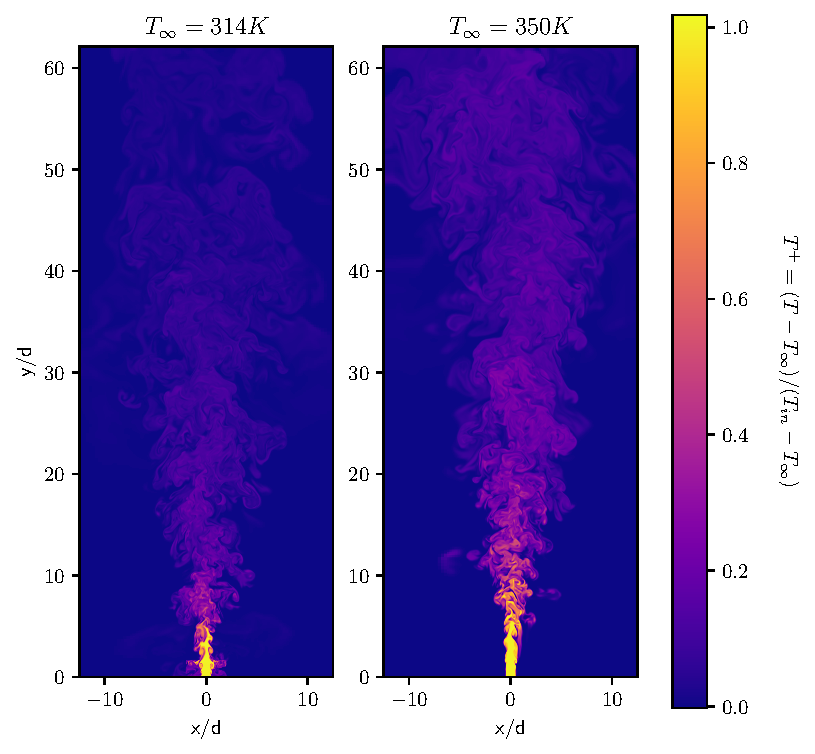
\includegraphics[scale=.45]{figures/Plots/vertical/temp_scaled_vert_noniso.pdf}
	\caption{Instantaneous temperature field.} \label{noniso_temp_1}
\end{subfigure}
\hfill
\begin{subfigure}{0.5\textwidth}
	\centering
	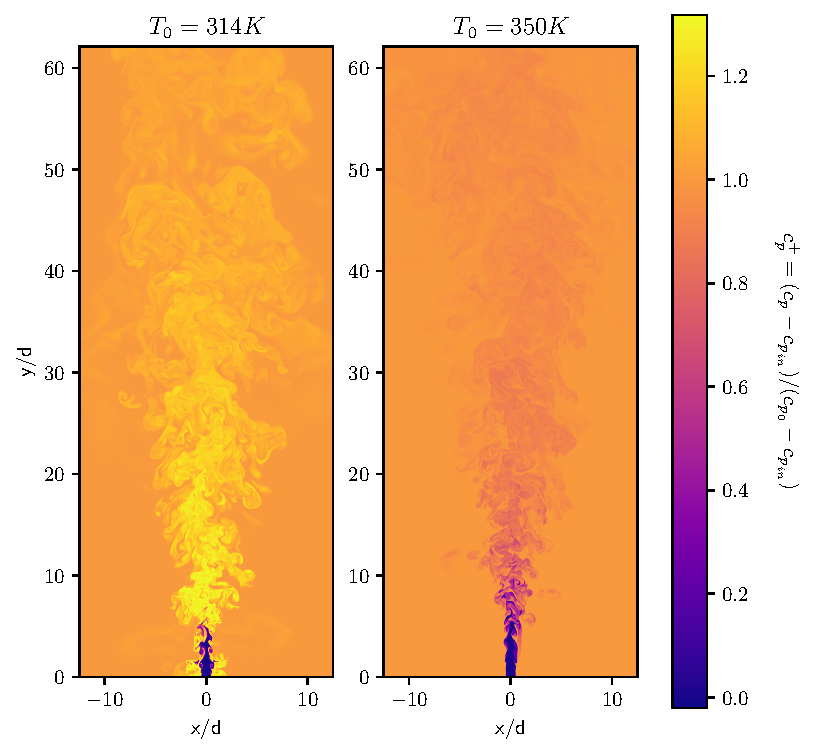
\includegraphics[scale=.45]{figures/Plots/vertical/cp_scaled_vert_noniso.pdf}
	\caption{Instantaneous constant pressure specific heat.} \label{noniso_cp_1}
\end{subfigure}
\vfill
\begin{subfigure}{0.5\textwidth}
	\centering
	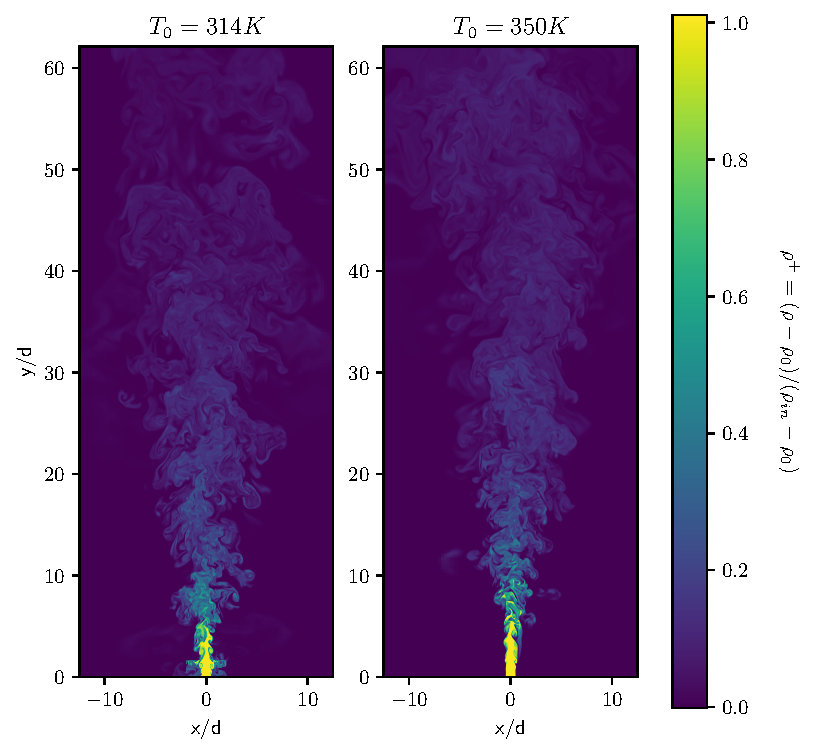
\includegraphics[scale=.45]{figures/Plots/vertical/rho_scaled_vert_noniso.pdf}
	\caption{Instantaneous density.} \label{noniso_rho_1}
\end{subfigure}
\hfill
\begin{subfigure}{0.5\textwidth}
	\centering
	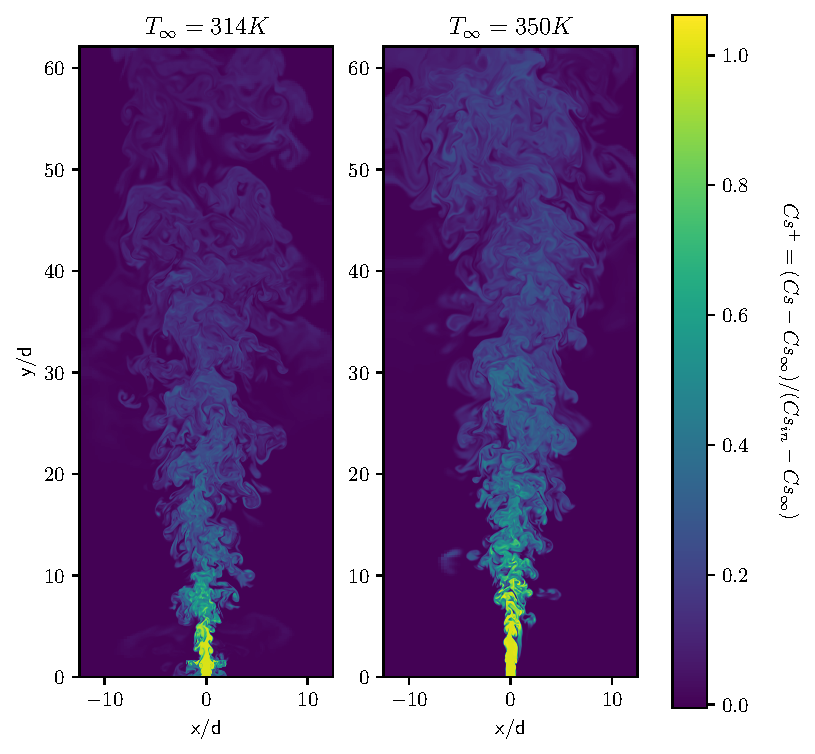
\includegraphics[scale=.45]{figures/Plots/vertical/Cs_scaled_vert_noniso.pdf}
	\caption{Instantaneous sound speed.} \label{noniso_Cs_1}
\end{subfigure}
\vfill
\begin{subfigure}{0.5\textwidth}
	\centering
	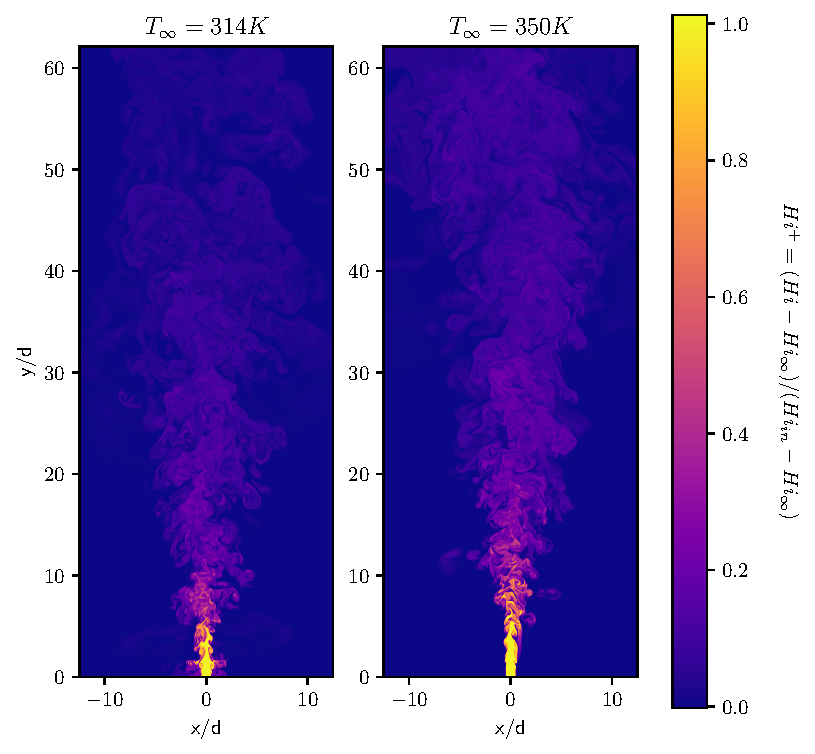
\includegraphics[scale=.45]{figures/Plots/vertical/Hi_scaled_vert_noniso.pdf}
	\caption{Instantaneous enthalpy.} \label{noniso_Hi_1}
\end{subfigure}
\hfill
\begin{subfigure}{0.5\textwidth}
	\centering
	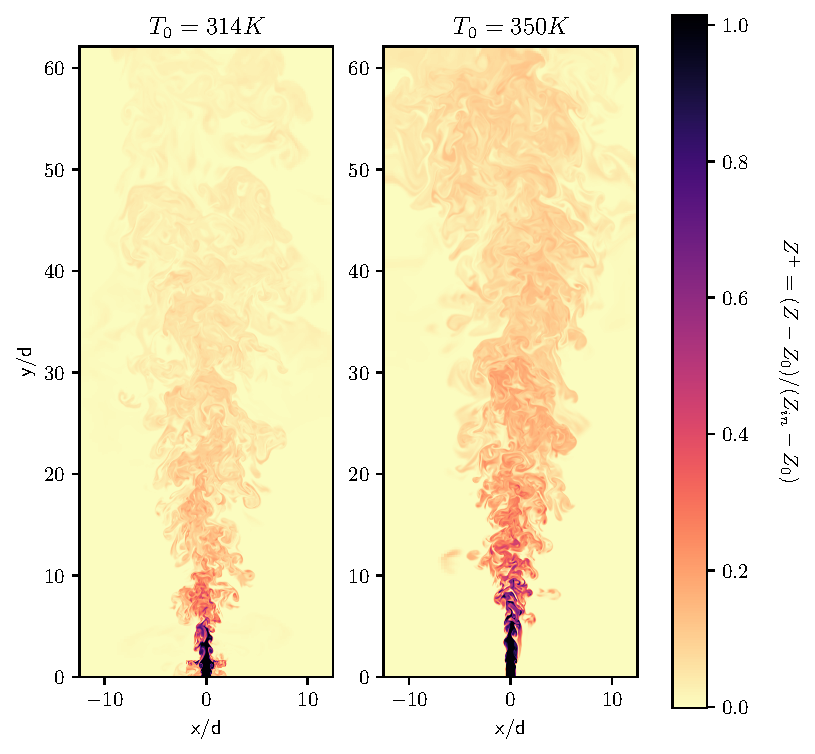
\includegraphics[scale=.45]{figures/Plots/vertical/Z_scaled_vert_noniso.pdf}
	\caption{Instantaneous compressibility factor} \label{noniso_Z_1}
\end{subfigure}
\caption{Direct comparison between 314K ambient case (left) and 350K ambient case (right) for various fluid quantities of interest.}
\label{noniso_various_features}
\end{figure}

\subsection{Mean Flow Properties}
Figure \ref{noniso_v_vin_r_d_features} depicts the time and radially averaged scaled axial velocity component plotted against radial distance from the centerline at multiple normal slices downstream from the inlet. The velocity is scaled by the average axial velocity value at the inflow while the radial direction is scaled by the jet diameter. In both cases, velocity profiles flatten as they get further downstream. Compared to the $330 K$ ambient case, the $350 K$ ambient case has a slower axial velocity decay downstream while the $314 K$ ambient case has a much faster decay. This agrees with the trends seen in the vertical slice images. 
\begin{figure}[H]
\begin{center}
\begin{subfigure}{0.45\textwidth}
	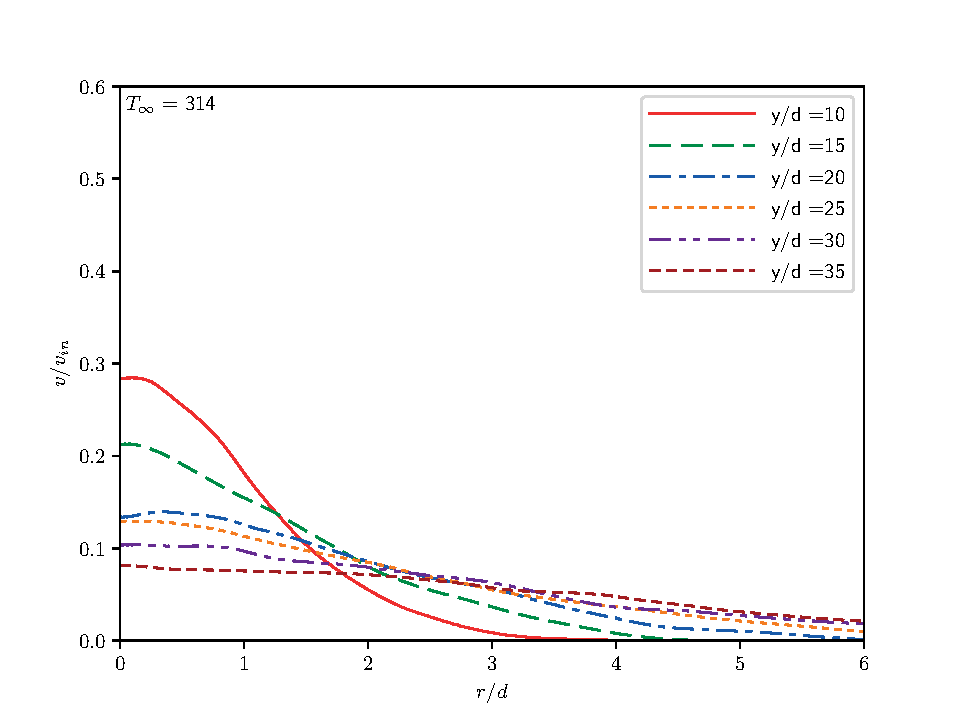
\includegraphics[scale=.45]{figures/Plots/radial/slices_5/314_ambient/ur_u_in_vs_r_d.pdf}
	\caption{314 K ambient case} \label{noniso_v_vin_r_d_1}
\end{subfigure}
\begin{subfigure}{0.45\textwidth}
	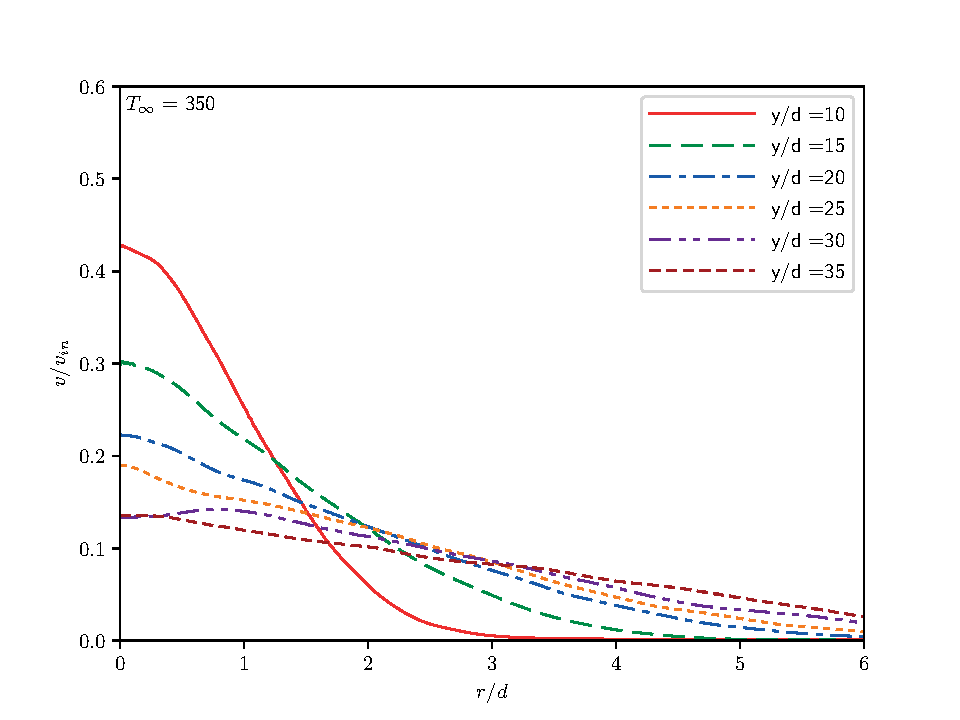
\includegraphics[scale=.45]{figures/Plots/radial/slices_5/350_ambient/ur_u_in_vs_r_d.pdf}
	\caption{350 K ambient case} \label{noniso_v_vin_r_d_2}
\end{subfigure}
\caption{Average (both in time and radially) axial velocity scaled by inlet value plotted along radial distance from centerline.}
\label{noniso_v_vin_r_d_features}
\end{center}
\end{figure}
Figures \ref{noniso_near_r_v_features} shows a different scaling of the axial velocity profiles depicted in the previous figure. Here, the axial velocity is scaled by the centerline value at each normal slice while the radial distance is scaled by the $r_{1/2}$, as was done in Figure \ref{330_r_v_features}. Figures \ref{noniso_near_r_vs_v_1} and \ref{noniso_near_r_vs_v_2} show the near field profiles resulting from this scaling. As was the case with the $330 K $ ambient case, self-similarity is seen in the near field for the non-isothermal cases, where fairly agreeable profile collapse occurs at $\nicefrac{y}{d} = 15$. The $350 K$ ambient case profiles are slightly more in-line with each other as compared to the $314 K$ ambient case, but both demonstrate a general tendency toward self-similarity still. Figures \ref{noniso_far_r_vs_v_1} and \ref{noniso_far_r_vs_v_2} however do not show as agreeable a collapse as the $330 K$ ambient case, though one still might be able to say the profiles tend toward self-similarity still. The $314 K$ ambient case has better self-similarity structure toward the centerline of the jet as compared to the $350 K$ ambient case, though the outer edge of the jet has a wider spread of profiles. The $350 K$ ambient case generally has a more uniform spread of profiles in both regions before and after the \gls{hmhw}. 
\begin{figure}[H]
\begin{center}
\begin{subfigure}{0.45\textwidth}
	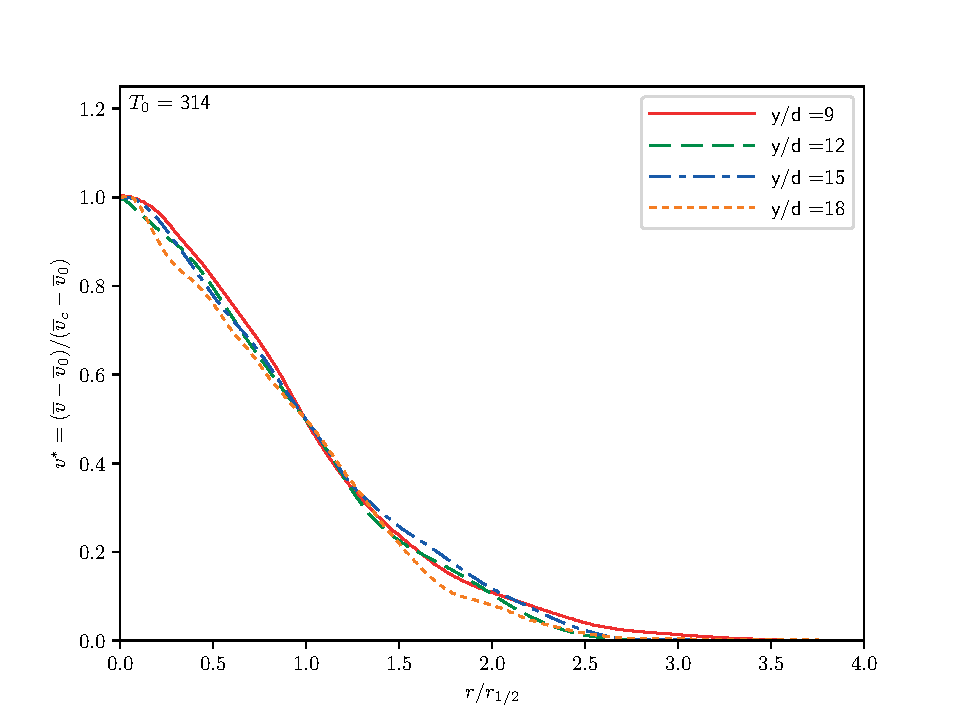
\includegraphics[scale=.45]{figures/Plots/radial/slices_3/314_ambient/r_vs_v.pdf}
	\caption{314 K ambient case in the near-field} \label{noniso_near_r_vs_v_1}
\end{subfigure}
\begin{subfigure}{0.45\textwidth}
	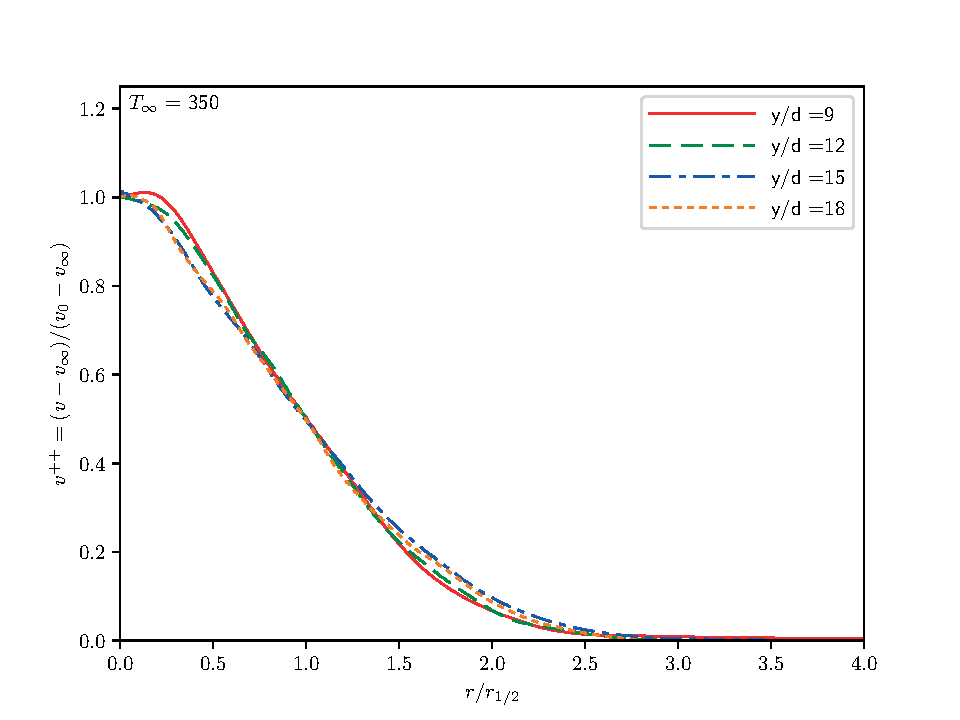
\includegraphics[scale=.45]{figures/Plots/radial/slices_3/350_ambient/r_vs_v.pdf}
	\caption{350 K ambient case in the near-field} \label{noniso_near_r_vs_v_2}
\end{subfigure}
\vfill
\begin{subfigure}{0.45\textwidth}
	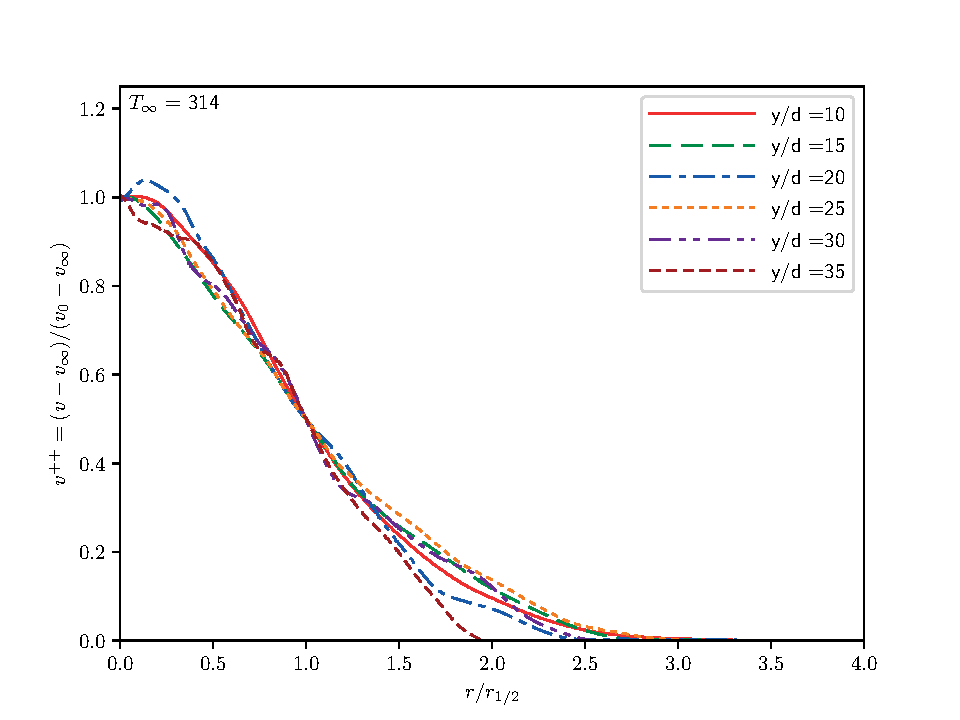
\includegraphics[scale=.45]{figures/Plots/radial/slices_5/314_ambient/r_vs_v.pdf}
	\caption{314 K ambient case in the far-field} \label{noniso_far_r_vs_v_1}
\end{subfigure}
\begin{subfigure}{0.45\textwidth}
	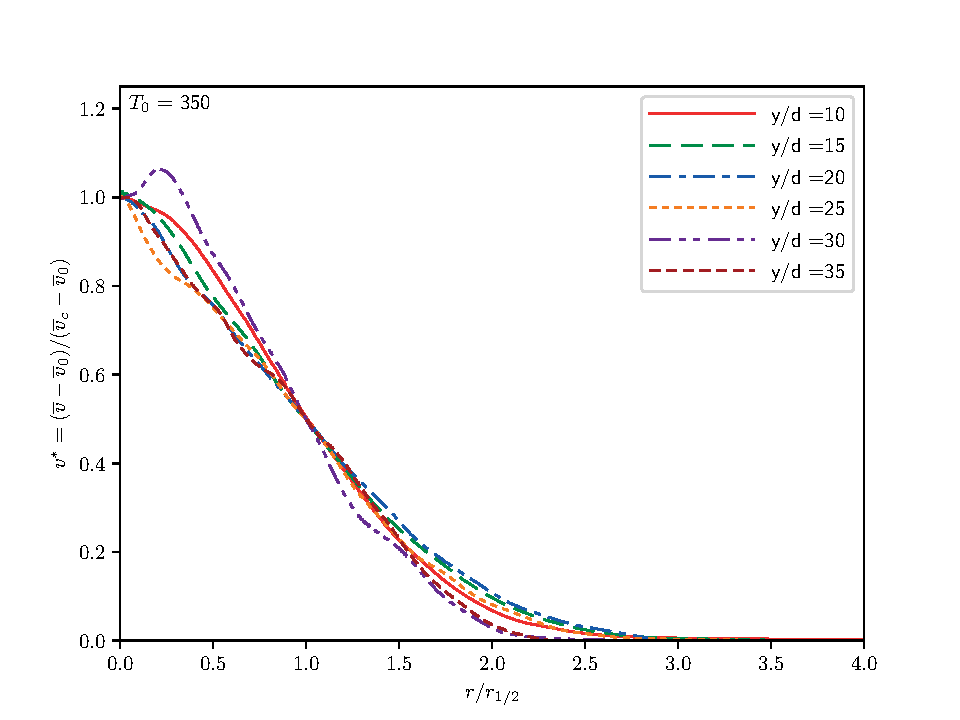
\includegraphics[scale=.45]{figures/Plots/radial/slices_5/350_ambient/r_vs_v.pdf}
	\caption{350 K ambient case in the far-field} \label{noniso_far_r_vs_v_2}
\end{subfigure}
\caption{Normal slices of scaled near-field and far-field axial velocity profiles, averaged in both time and the radial direction. Plotted against radial direction scaled by $r_{1/2}$.}
\label{noniso_near_r_v_features}
\end{center}
\end{figure}
%\begin{figure}[htbp!]
%\begin{center}
%\begin{subfigure}{0.45\textwidth}
%	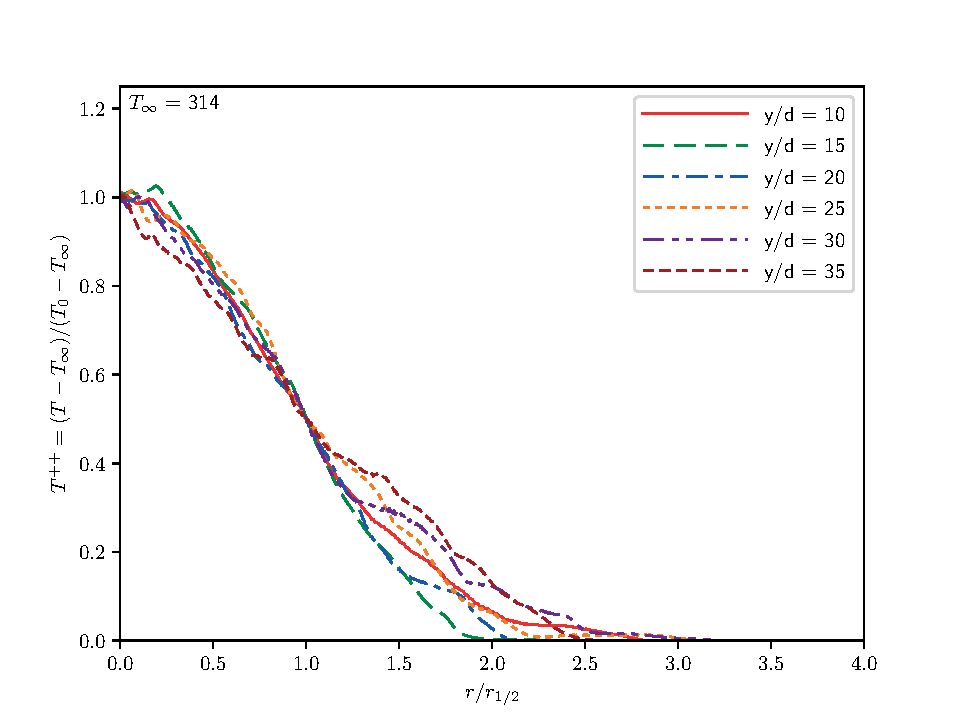
\includegraphics[scale=.45]{figures/Plots/radial/slices_5/314_ambient/r_vs_temp.pdf}
%	\caption{314 K ambient case} \label{noniso_r_vs_temp_1}
%\end{subfigure}
%\begin{subfigure}{0.45\textwidth}
%	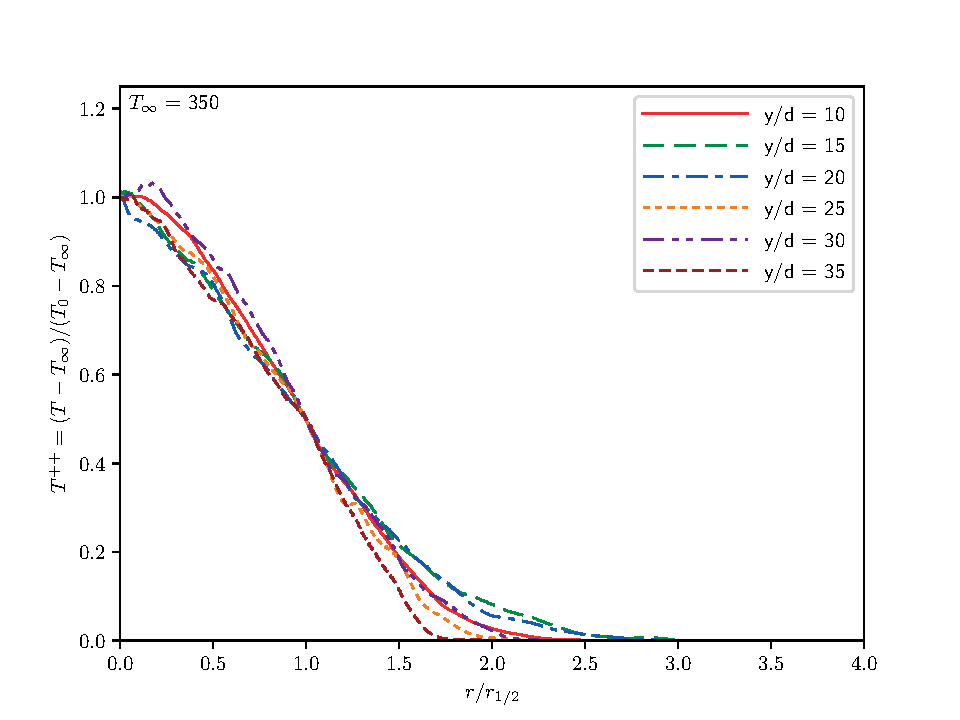
\includegraphics[scale=.45]{figures/Plots/radial/slices_5/350_ambient/r_vs_temp.pdf}
%	\caption{350 K ambient case} \label{noniso_r_vs_temp_2}
%\end{subfigure}
%\caption{Normal slices of scaled far-field temperature, averaged in both time and the radial direction. Plotted against radial direction scaled by $r_{1/2}$.}
%\label{noniso_far_r_temp_features}
%\end{center}
%\end{figure}
Density self-similarity is not as evident as is in axial velocity profiles, as can be seen in Figure \ref{noniso_far_r_rho_features}. The $350 K$ ambient case shows more promise but the profile spread is not nearly as tight as it was with the axial velocity. The $314 K$ case is even worse, with more prominent fluctuations in the curves than any of the previous profile depictions. Far-field density in this case has the widest spread of all previous comparisons. One interesting feature of these plots can be seen on the outer edge of the jet, past the \gls{hmhw} mark. For the $314 K$ ambient case, profiles exhibit an initial decay as they dip below the $\nicefrac{y}{d}=10$ profile before increasing to fall above this initial curve at later slices downstream. This is opposite to what is seen in the $350 K$ ambient case, where earlier slices rise above the initial curve at $\nicefrac{y}{d} = 10$ before decaying below it further downstream. This later decay is consistent with what is seen in the axial velocity self-similarity curves for both cases, while the density profiles for the $314 K$ ambient case break from this pattern. 
\begin{figure}[H]
\begin{center}
\begin{subfigure}{0.45\textwidth}
	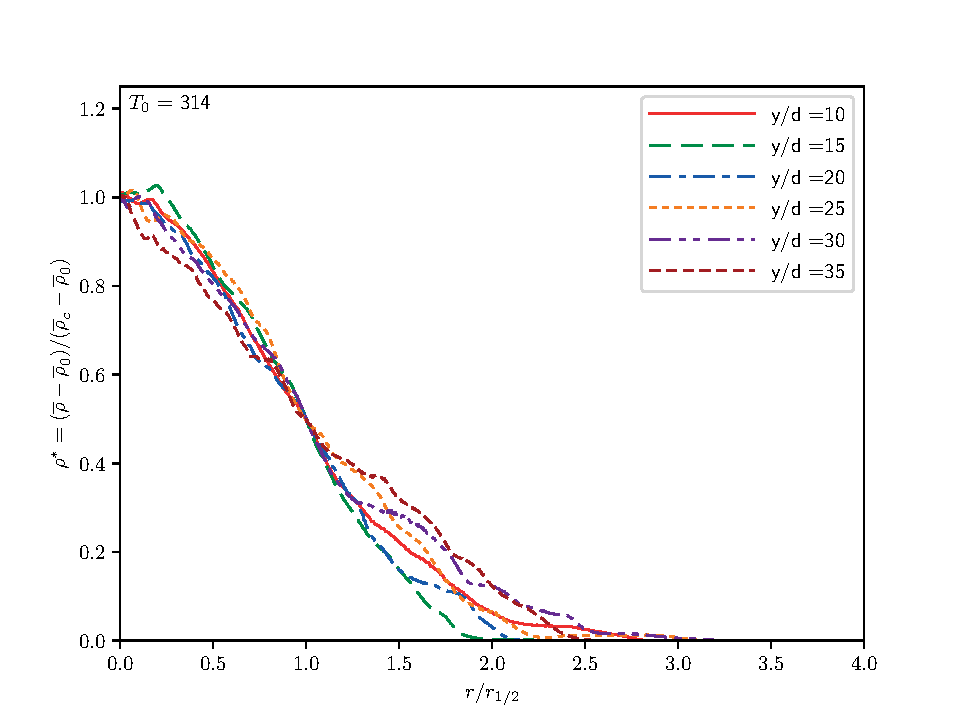
\includegraphics[scale=.45]{figures/Plots/radial/slices_5/314_ambient/r_vs_rho.pdf}
	\caption{314 K ambient case} \label{noniso_r_vs_rho_1}
\end{subfigure}
\begin{subfigure}{0.45\textwidth}
	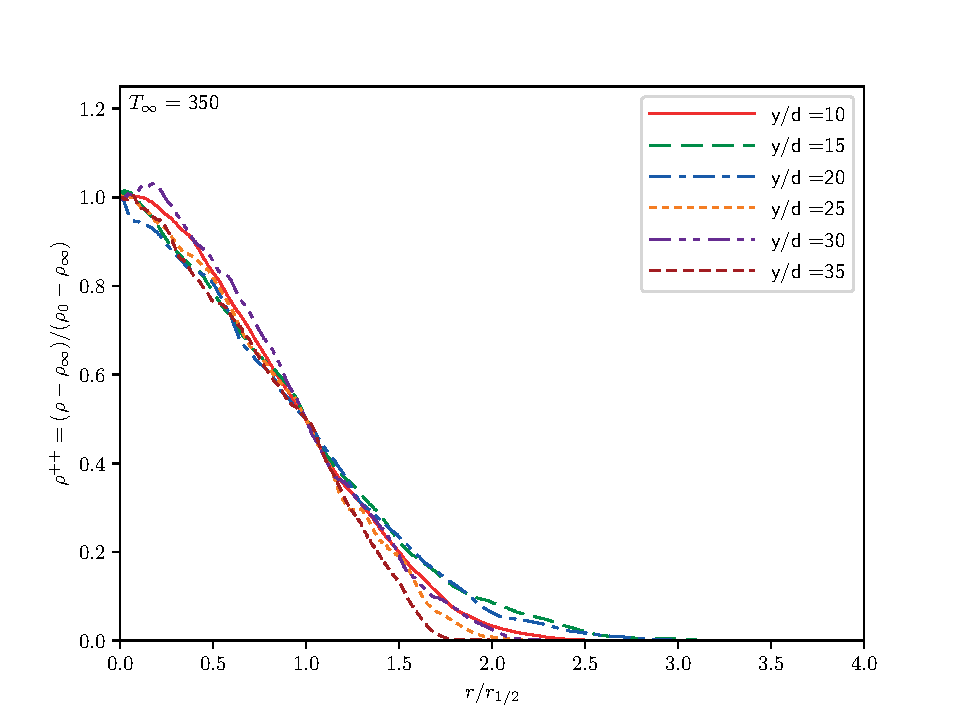
\includegraphics[scale=.45]{figures/Plots/radial/slices_5/350_ambient/r_vs_rho.pdf}
	\caption{350 K ambient case} \label{noniso_r_vs_rho_2}
\end{subfigure}
\caption{Normal slices of scaled far-field density, averaged in both time and the radial direction. Plotted against radial direction scaled by $r_{1/2}$.}
\label{noniso_far_r_rho_features}
\end{center}
\end{figure}
Figure \ref{noniso_uin_u0_x_d_features} shows the recovery of linear decay in the axial velocity along the centerline of the jet for each case. The $350 K$ ambient case has a less steep slope compared to the $330 K$ ambient case seen in Figure \ref{330_centerline_scaling}, corresponding to a slower decay in axial velocity along the centerline. The $314 K$ ambient case has a steeper slope compared to the $330 K$ ambient case, which corresponds to the centerline decay occurring at a faster rate than that in the base case. These findings are consistent with the analysis from Figure \ref{noniso_v_vin_r_d_features}.
\begin{figure}[H]
\begin{center}
\begin{subfigure}{0.45\textwidth}
	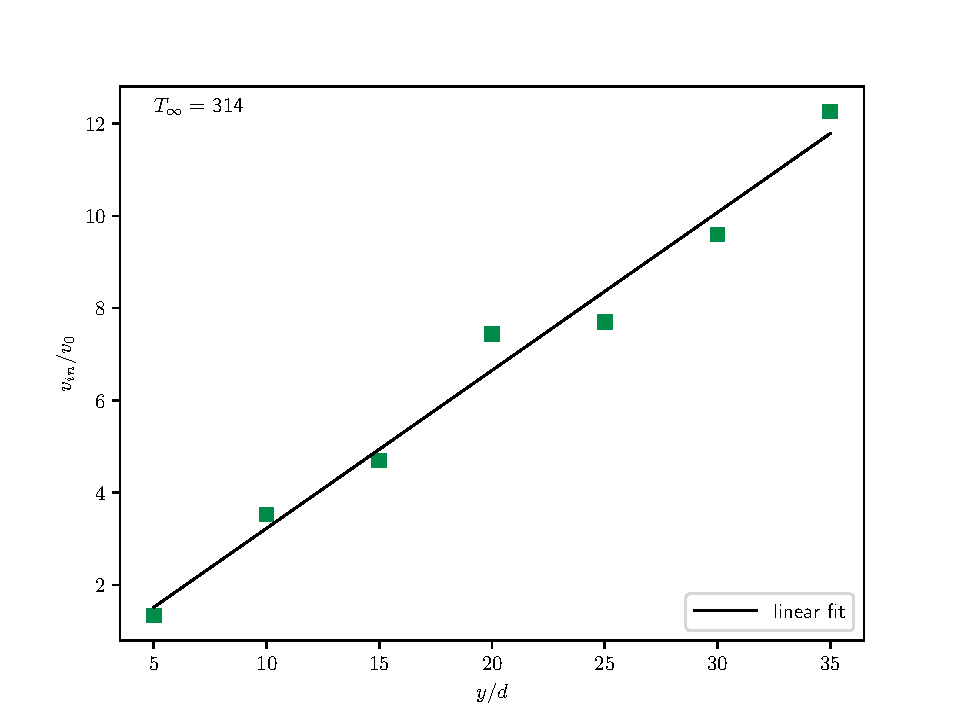
\includegraphics[scale=.45]{figures/Plots/radial/slices_5/314_ambient/uin_u0_vs_x_d.pdf}
	\caption{314 K ambient case} \label{noniso_uin_u0_x_c_1}
\end{subfigure}
\begin{subfigure}{0.45\textwidth}
	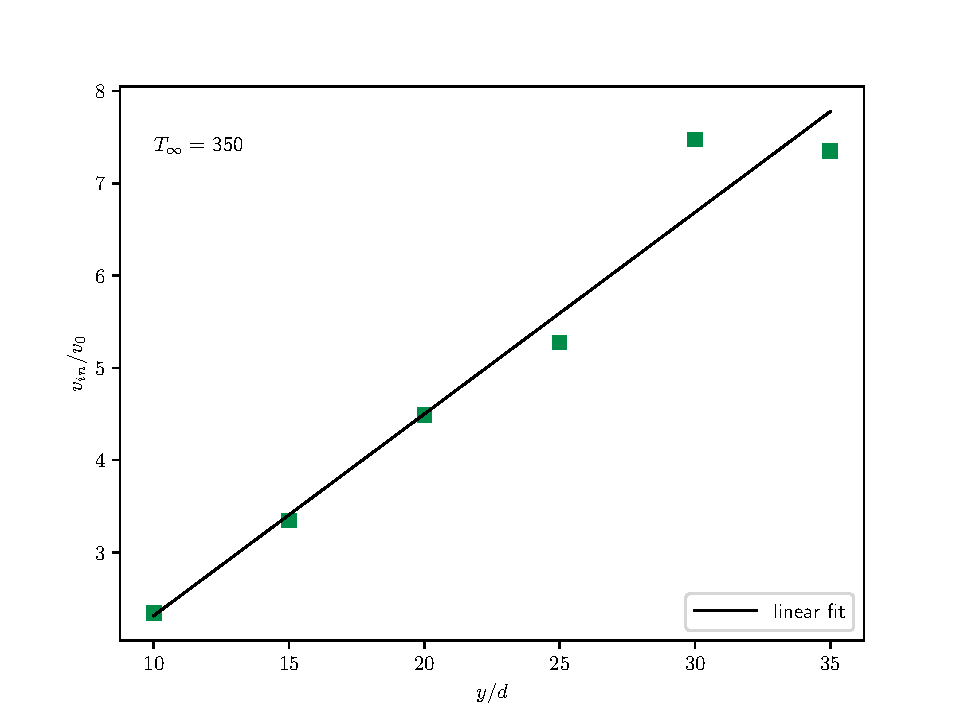
\includegraphics[scale=.45]{figures/Plots/radial/slices_5/350_ambient/uin_u0_vs_x_d.pdf}
	\caption{350 K ambient case} \label{noniso_uin_u0_x_d_2}
\end{subfigure}
\caption{Axial inlet velocity scaled by centerline values along the axial direction. When distance downstream is scaled by jet diameter, linear decay of the centerline axial velocity is observed.}
\label{noniso_uin_u0_x_d_features}
\end{center}
\end{figure}
Finally, Figure \ref{noniso_centerline_features} shows various quantities along the centerline for both non-isothermal cases. For all quantities presented here, centerline plots help depict the different regions of the jet. The potential core is maintained until around $\nicefrac{y}{d} = 2.5$ for the $314 K$ ambient case and until around $\nicefrac{y}{d}= 5$ for the $350 K$ ambient case. Then there is a transition region where quantities experience rapid change. This occurs up until about $\nicefrac{y}{d}= 10$ for the $314 K$ ambient case and $\nicefrac{y}{d} = 12$ for the $350 K$ ambient case. After that, a gradual leveling out occurs as the quantity of interest continues to adjust as it mixes with the ambient fluid through the remainder of the domain. Figure \ref{noniso_temp_centerline_1} shows the temperature change for each case along the centerline of the jet. The $314 K$ ambient case exhibits a more rapid decay from the inflow temperature as compared to the $350 K$ ambient case, as can be seen in the separation between the curves between $4 \leq \nicefrac{y}{d} \leq 16$. Afterwards, they continue their respective transition toward ambient conditions at roughly the same rate. The $350 K$ ambient case never gets as close to ambient conditions as the $314 K$ ambient case due to the slower initial decline, hovering instead around $T^+=0.18$ as compared to the $T^+=0.14$ that the $314 K$ ambient case sits at. Enthalpy and the compressibility factor in Figures \ref{noniso_Hi_centerline_1} and \ref{noniso_Z_centerline_1} respectively follow the same trend though with less separation between the two cases as compared to the temperature trajectories. Figure \ref{noniso_Cs_centerline_1} shows the sound speed transition along the centerline. Compared to the previously discussed quantities, the sound speed decay appears much more gradual, with little rate difference between the two cases. The initial transition region is less steep and the region thereafter more of a continued gradual decline as opposed to a leveling out like the other quantities. Figure \ref{noniso_cp_centerline_1} shows the constant-pressure specific heat for the two non-isothermal cases. Again, neither fully transitions to the ambient condition as the jet persists through the domain. Here the jump in specific heat over the peak present near the pseudo-boiling point can be seen for the $314 K$ ambient case. This case also has a steeper initial transition than the other case does, though both have similar rates of approach toward ambient conditions after this initial shift. Figure \ref{noniso_rho_centerline_1} shows the density of the two cases. This quantity follows a unique trajectory between the two cases compared to those previously discussed. Here, the initial transition rate of the two cases from the potential core to the fully developed region is nearly the same for the most part. Toward the end of this transition though,  the $314 K$ ambient case begins to level out at a faster rate than the $350 K$ ambient case, allowing the curves to collapse onto each other. Then both centerline densities continue on past $\nicefrac{y}{d} = 16$ at approximately $\rho^+ = .12$ and steadily decline toward ambient conditions thereafter. 
\begin{figure}[H]
\begin{center}
\begin{subfigure}{0.45\textwidth}
	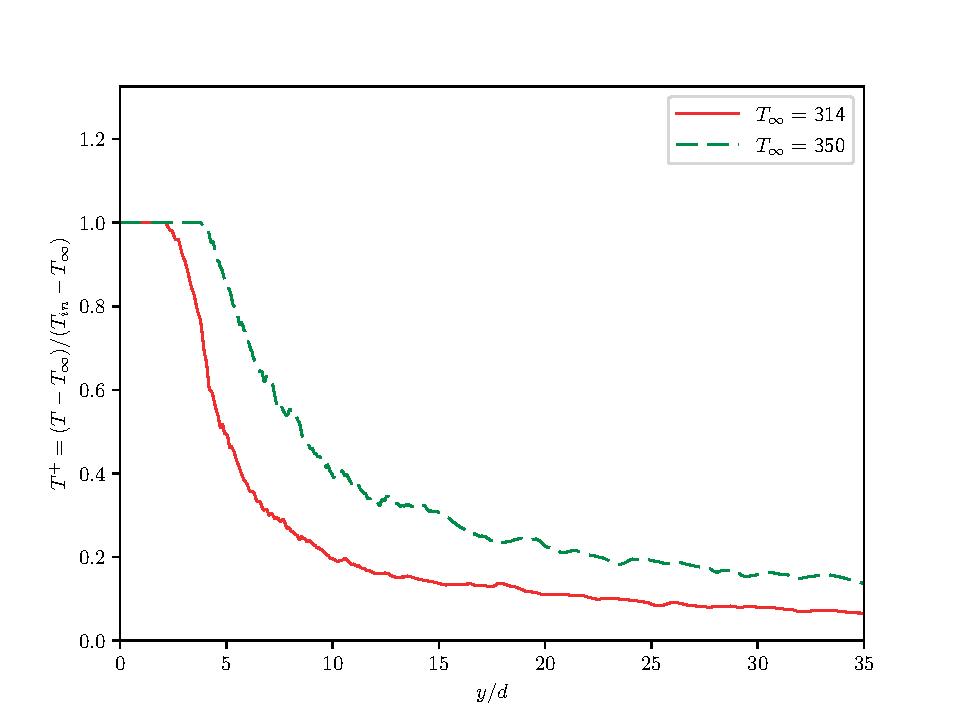
\includegraphics[scale=.45]{figures/Plots/centerline/temp_centerline_scaled.pdf}
	\caption{Temperature} \label{noniso_temp_centerline_1}
\end{subfigure}
\begin{subfigure}{0.45\textwidth}
	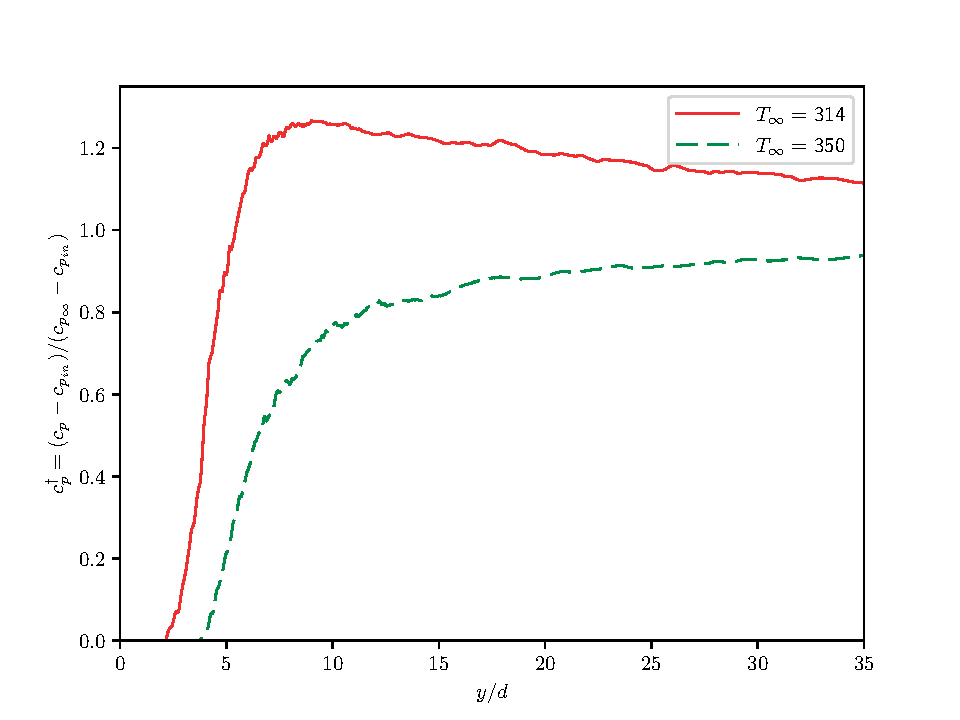
\includegraphics[scale=.45]{figures/Plots/centerline/cp_centerline_scaled.pdf}
	\caption{Constant-pressure specific heat} \label{noniso_cp_centerline_1}
\end{subfigure}
\vfill
\begin{subfigure}{0.45\textwidth}
	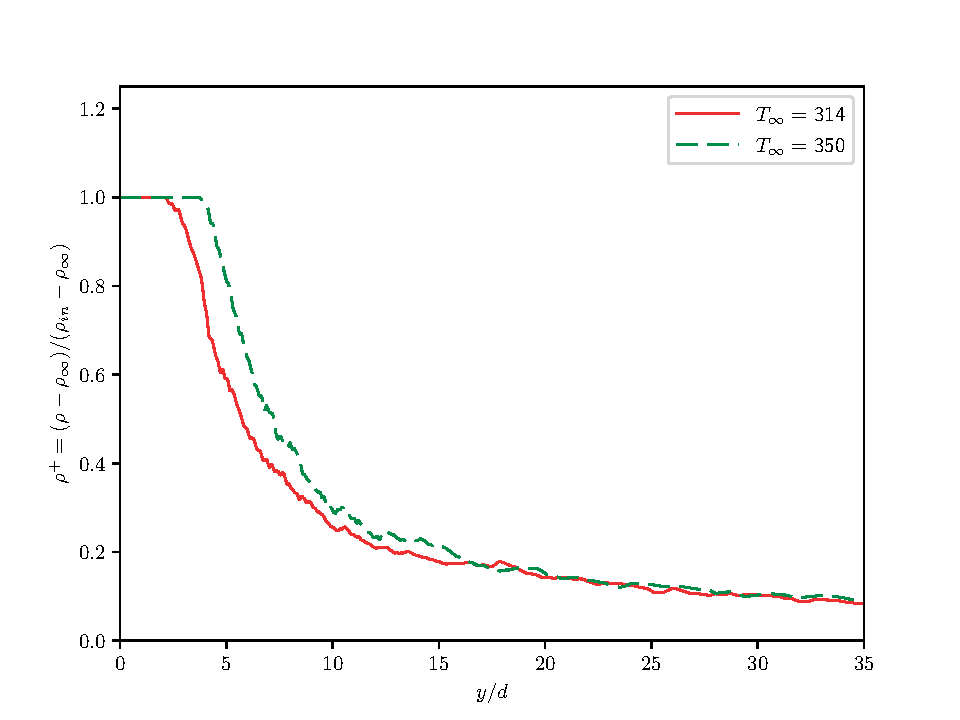
\includegraphics[scale=.45]{figures/Plots/centerline/rho_centerline_scaled.pdf}
	\caption{Density} \label{noniso_rho_centerline_1}
\end{subfigure}
\begin{subfigure}{0.45\textwidth}
	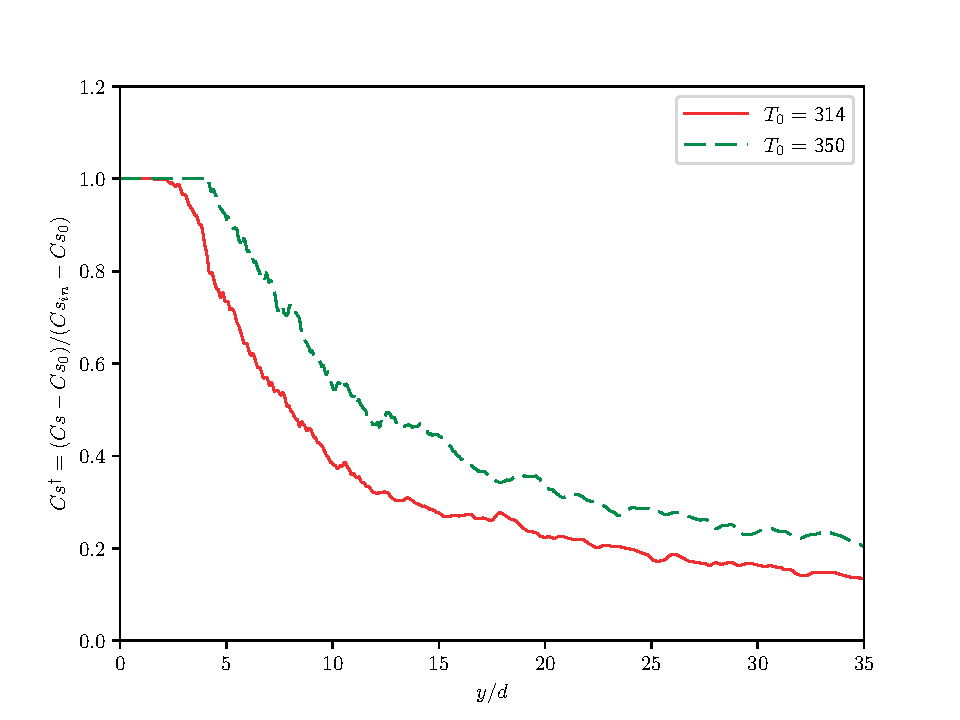
\includegraphics[scale=.45]{figures/Plots/centerline/Cs_centerline_scaled.pdf}
	\caption{Sound speed} \label{noniso_Cs_centerline_1}
\end{subfigure}
\vfill
\begin{subfigure}{0.45\textwidth}
	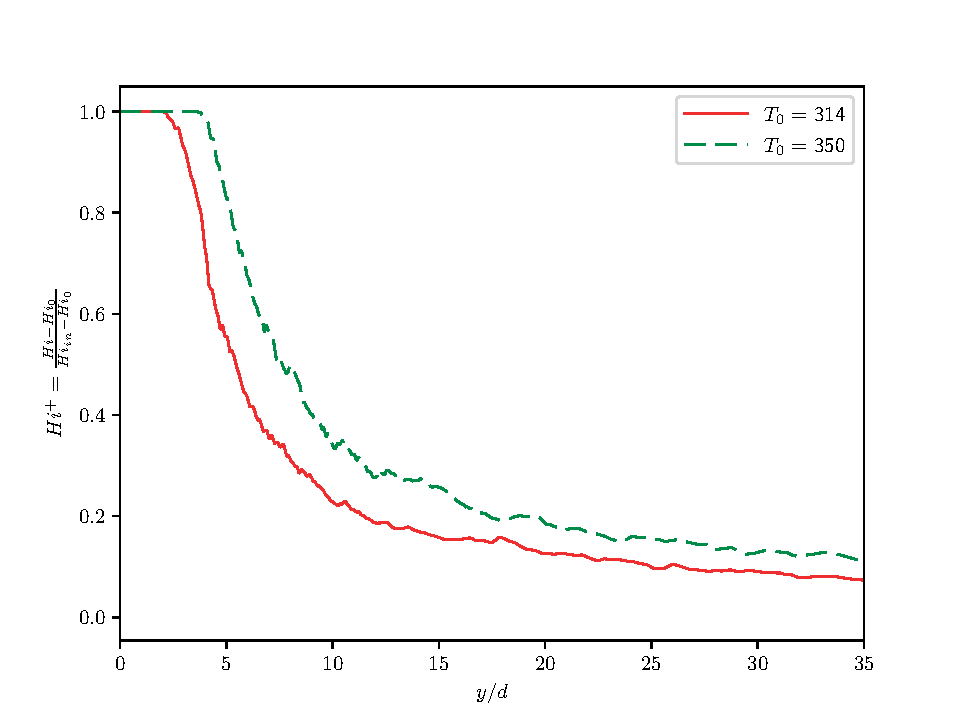
\includegraphics[scale=.45]{figures/Plots/centerline/Hi_centerline_scaled.pdf}
	\caption{Enthalpy} \label{noniso_Hi_centerline_1}
\end{subfigure}
\begin{subfigure}{0.45\textwidth}
	\includegraphics[scale=.45]{figures/Plots/centerline/Z_centerline_scaled.pdf}
	\caption{Compressibility Factor} \label{noniso_Z_centerline_1}
\end{subfigure}

\caption{Comparison of centerline decay for various fluid quantities.}
\label{noniso_centerline_features}
\end{center}
\end{figure}

\subsection{Turbulence Dynamics}
Figure \ref{noniso_reynolds_features} shows the resolved Reynolds stresses of each non-isothermal case at two different locations downstream. As was the case with the $330 K$ ambient resolved Reynolds stresses in Figure \ref{330_reynolds_features}, self-similarity in the axial direction is not recovered. The Reynolds stresses for both of the non-isothermal cases are generally smaller than their counterparts in the isothermal case. The stresses in Figure \ref{350_rey_15} generally follow the trends outlined in the isothermal case, but the remaining slices for these two cases do not follow suite, with little to no separation between the axial direction stresses and the other stresses. This could be due the effects of the \gls{sgs} modeling as mentioned in \cite{doi:10.1063/1.4937948}.  
\begin{figure}[ht!]
\begin{center}
\begin{subfigure}{0.45\textwidth}
	\includegraphics[scale=.45]{figures/Plots/radial/slices_5/314_ambient/Rey_Stress_0_15.pdf}
	\caption{Reynolds stresses at $y/d=15$ for 314 K ambient case} \label{314_rey_15}
\end{subfigure}
\begin{subfigure}{0.45\textwidth}
	\includegraphics[scale=.45]{figures/Plots/radial/slices_5/350_ambient/Rey_Stress_0_15.pdf}
	\caption{Reynolds stresses at $y/d=15$ for 350 K ambient case} \label{350_rey_15}
\end{subfigure}
\vfill
\begin{subfigure}{0.45\textwidth}
	\includegraphics[scale=.45]{figures/Plots/radial/slices_5/314_ambient/Rey_Stress_0_2.pdf}
	\caption{Reynolds stresses at $y/d=20$ for 314 K ambient case} \label{314_rey_20}
\end{subfigure}
\begin{subfigure}{0.45\textwidth}
	\includegraphics[scale=.45]{figures/Plots/radial/slices_5/350_ambient/Rey_Stress_0_2.pdf}
	\caption{Reynolds stresses at $y/d=20$ for 350 K ambient case} \label{350_rey_20}
\end{subfigure}
\caption{Time and radially averaged Reynolds stresses for the non-isothermal jets at two locations downstream.}
\label{noniso_reynolds_features}
\end{center}
\end{figure}

Figure \ref{noniso_TKE_component_features} shows the components of the resolved \gls{tke} for each non-isothermal case. Both cases follow the same general trends seen in the $330 K$ ambient case, with the axial component being the strongest and the other two components being of the same magnitude. The $350 K$ ambient case is the most similar to the $330 K$ ambient case between the two. For this case, peak \gls{tke} occurs at approximately $\nicefrac{y}{d} = 7$, which is slightly later than the isothermal case. Additionally, this peak is aligned with the peak seen in the other components, where for the isothermal case the axial component peak came slightly before the peak of the other two. Magnitude of the peak axial component is larger in the $350 K$ ambient case while the magnitudes of the other directional components are similar to their counterparts in the $330 K$ ambient case. Decay rate is also slightly higher in the $350 K$ ambient case compared to the isothermal case. The \gls{tke} components of the $314 K$ ambient case reach their peaks slightly earlier than the $330 K$ ambient case at about $\nicefrac{y}{d} = 5$. The peak of the axial component is much larger than that of the other two cases. Additionally, the other \gls{tke} components of the $314 K$ ambient case have a smaller magnitude than their counterparts in the other cases, resulting in a larger disparity between the magnitudes of the components in this case. There is also stronger overall decay in the $314 K$ ambient case as compared to the $350 K$ ambient case.

\begin{figure}[ht!]
\begin{center}
\begin{subfigure}{0.45\textwidth}
	\includegraphics[scale=.45]{figures/Plots/centerline/314_TKEuvw_centerline.pdf}
	\caption{314 K ambient case} \label{314_TKEcomp_1}
\end{subfigure}
\begin{subfigure}{0.45\textwidth}
	\includegraphics[scale=.45]{figures/Plots/centerline/350_TKEuvw_centerline.pdf}
	\caption{350 K ambient case} \label{350_TKEcomp_1}
\end{subfigure}
\caption{Comparison of average turbulent kinetic energy components along centerline for each non-isothermal case.}
\label{noniso_TKE_component_features}
\end{center}
\end{figure}

Figure \ref{noniso_TKE_features} further emphasizes the differences between the \gls{tke} components and overall \gls{tke} by directly comparing each quantity across all cases. For all quantities, the $314 K$ ambient case peaks before the other two cases. For the overall resolved \gls{tke} and the axial component, the $330 K$ ambient case is next to peak, followed by the $350 K$ ambient case. For the cross directional components, the peaks of these two cases coincide. The $314 K$ ambient cases experiences the strongest decay along the centerline immediately following the peak for each quantity, however, the other two cases eventually decay to the same value so that all cases exhibit a roughly equivalent leveling off as the jet progresses through the remainder of the domain. 

\begin{figure}[H]
\begin{center}
\begin{subfigure}{0.45\textwidth}
	\includegraphics[scale=.45]{figures/Plots/centerline/TKE_centerline.pdf}
	\caption{Resolved Turbulent Kinetic Energy} \label{TKE_centerline_1}
\end{subfigure}
\begin{subfigure}{0.45\textwidth}
	\includegraphics[scale=.45]{figures/Plots/centerline/u_fa_centerline.pdf}
	\caption{u-directional TKE component} \label{u_fa_1}
\end{subfigure}
\vfill
\begin{subfigure}{0.45\textwidth}
	\includegraphics[scale=.45]{figures/Plots/centerline/v_fa_centerline.pdf}
	\caption{v-directional TKE component} \label{v_fa_1}
\end{subfigure}
\begin{subfigure}{0.45\textwidth}
	\includegraphics[scale=.45]{figures/Plots/centerline/w_fa_centerline.pdf}
	\caption{w-directional TKE component} \label{w_fa_1}
\end{subfigure}
\caption{Cross-case comparisons of average turbulent kinetic energy components and total resolved TKE along centerline.}
\label{noniso_TKE_features}
\end{center}
\end{figure}



% \section{Discussion}





